\documentclass[pdflatex,sn-mathphys-ay]{sn-jnl}

\usepackage[T1]{fontenc}%
\usepackage{graphicx}%
\usepackage{multirow}%
\usepackage{amsmath,amssymb,amsfonts}%
\usepackage{amsthm}%
\usepackage{mathrsfs}%
\usepackage[title]{appendix}%
\usepackage{xcolor}%
\usepackage{textcomp}%
\usepackage{manyfoot}%
\usepackage{booktabs}%
\usepackage{array}%
\usepackage{longtable}%
\usepackage{calc}%
\usepackage{newunicodechar}%
\usepackage{fvextra}%
\providecommand{\tightlist}{\setlength{\itemsep}{0pt}\setlength{\parskip}{0pt}}
\providecommand{\lt}{<}\providecommand{\gt}{>}
\newunicodechar{§}{\S}
\newunicodechar{→}{\ensuremath{\rightarrow}}
\newunicodechar{↔}{\ensuremath{\leftrightarrow}}
\newunicodechar{×}{\ensuremath{\times}}
\newunicodechar{·}{\ensuremath{\cdot}}
\newunicodechar{⊃}{\ensuremath{\supset}}
\newunicodechar{°}{\ensuremath{^{\circ}}}
\newunicodechar{₀}{\textsubscript{0}}\newunicodechar{₁}{\textsubscript{1}}%
\newunicodechar{₂}{\textsubscript{2}}\newunicodechar{₃}{\textsubscript{3}}%
\newunicodechar{₄}{\textsubscript{4}}\newunicodechar{₅}{\textsubscript{5}}%
\newunicodechar{₆}{\textsubscript{6}}\newunicodechar{₇}{\textsubscript{7}}%
\newunicodechar{₈}{\textsubscript{8}}\newunicodechar{₉}{\textsubscript{9}}%
\newunicodechar{⁰}{\textsuperscript{0}}\newunicodechar{¹}{\textsuperscript{1}}%
\newunicodechar{²}{\textsuperscript{2}}\newunicodechar{³}{\textsuperscript{3}}%
\newunicodechar{⁴}{\textsuperscript{4}}\newunicodechar{⁵}{\textsuperscript{5}}%
\newunicodechar{⁶}{\textsuperscript{6}}\newunicodechar{⁷}{\textsuperscript{7}}%
\newunicodechar{⁸}{\textsuperscript{8}}\newunicodechar{⁹}{\textsuperscript{9}}%
\newunicodechar{⁻}{\textsuperscript{-}}\newunicodechar{≈}{\ensuremath{\approx}}%
\newunicodechar{≤}{\ensuremath{\le}}\newunicodechar{≥}{\ensuremath{\ge}}%
\newunicodechar{∼}{\ensuremath{\sim}}\newunicodechar{−}{\ensuremath{-}}%
\newunicodechar{∗}{\ensuremath{\ast}}\newunicodechar{∞}{\ensuremath{\infty}}%
\newunicodechar{τ}{\ensuremath{\tau}}\newunicodechar{ν}{\ensuremath{\nu}}%
\newunicodechar{λ}{\ensuremath{\lambda}}\newunicodechar{σ}{\ensuremath{\sigma}}%
\newunicodechar{α}{\ensuremath{\alpha}}\newunicodechar{η}{\ensuremath{\eta}}%
\newunicodechar{π}{\ensuremath{\pi}}\newunicodechar{μ}{\ensuremath{\mu}}\newunicodechar{ρ}{\ensuremath{\rho}}%
\newunicodechar{θ}{\ensuremath{\theta}}\newunicodechar{β}{\ensuremath{\beta}}\newunicodechar{γ}{\ensuremath{\gamma}}%
\newunicodechar{δ}{\ensuremath{\delta}}\newunicodechar{ε}{\ensuremath{\varepsilon}}\newunicodechar{κ}{\ensuremath{\kappa}}%
\newunicodechar{ξ}{\ensuremath{\xi}}\newunicodechar{ω}{\ensuremath{\omega}}\newunicodechar{χ}{\ensuremath{\chi}}%
\newunicodechar{ψ}{\ensuremath{\psi}}\newunicodechar{φ}{\ensuremath{\varphi}}\newunicodechar{Δ}{\ensuremath{\Delta}}%
\newunicodechar{Σ}{\ensuremath{\Sigma}}\newunicodechar{Π}{\ensuremath{\Pi}}\newunicodechar{Ω}{\ensuremath{\Omega}}%
\newunicodechar{Γ}{\ensuremath{\Gamma}}\newunicodechar{Λ}{\ensuremath{\Lambda}}\newunicodechar{Θ}{\ensuremath{\Theta}}%
\newunicodechar{«}{``}
\newunicodechar{»}{''}

\raggedbottom

\begin{document}

\title[Supplementary Material]{Supplementary Material: Informational Nostalgia}

\author*[1]{\fnm{Alexander} \sur{Andriishin}}\email{alexander@andriishin.com}

\affil*[1]{\orgname{Independent Researcher}, \orgaddress{\city{Moscow}, \country{Russia}}}

\maketitle

\section*{S1. Full proof of Remark 6 (softmax-regularity for OU)}\label{s1.-full-proof-of-remark-6-softmax-regularity-for-ou}



Remark 6 (§ 4.4) states: in the OU-class of § 5.2 the exponential decorrelation of the autocovariance of the logits \(\theta_v(t)\) is carried through the softmax to any bounded measurable functional \(\xi(\theta_v)\) (in particular, to the entries of the transition matrix \(P_{ij}(\theta_v)\) and to any sufficient prediction statistic; the covariance of \(\xi\) then decays with characteristic time \(\tau_E\), whereas the conditional MI decays twice as fast, with \(\tau_E/2\), since \(I \approx \tfrac{1}{2}\rho^2\) at small correlation, see S1.5a). The proof has five steps: (i) Lipschitz softmax in \(\ell_\infty\); (ii) transfer to the TV of the transition matrix; (iii) boundedness of the OU trajectory on a ball \(R(\delta)\) with probability \(1-\delta\); (iv) transfer of the decay to the covariance of \(\xi\); (v) translation of the TV bound into a bound on the conditional MI.



\subsection*{S1.1 Step 1. Lipschitz continuity of softmax}\label{s1.1-step-1.-lipschitz-continuity-of-softmax}



Let \(\text{softmax}: \mathbb{R}^k \to \Delta^{k-1}\) be the standard map \(\text{softmax}_i(\theta_v) = \exp\theta_i / \sum_j \exp\theta_j\). The Jacobian has the form \(\partial \text{softmax}_i / \partial \theta_j = \text{softmax}_i(\delta_{ij} - \text{softmax}_j)\); the diagonal entries \(p_i(1-p_i) \ge 0\), the off-diagonal ones \(-p_i p_j \le 0\), and the column sum of absolute values does not exceed \(2 p_j\). The standard consequence is the \(\ell_1 / \ell_\infty\) pairing estimate:



\begin{equation}\|\text{softmax}(\theta_v) - \text{softmax}(\theta_v')\|_1 \;\le\; 2 \, \|\theta_v - \theta_v'\|_\infty. \tag{S1.1}\end{equation}



\emph{Derivation of (S1.1) via the operator norm of the Jacobian.} The Jacobian \(J(\theta_v) = \text{diag}(p) - p p^T\) (where \(p = \text{softmax}(\theta_v)\)) is estimated in the induced \(\ell_\infty \to \ell_1\) norm: for any \(v\) with \(\|v\|_\infty \le 1\)



\[\|J v\|_1 = \sum_i \Bigl|\sum_j J_{ij} v_j\Bigr| \;\le\; \sum_i \sum_j |J_{ij}| \;=\; \sum_j \Bigl(\sum_i |J_{ij}|\Bigr),\]



and the column sum of absolute values equals \(|J_{jj}| + \sum_{i \ne j}|J_{ij}| = p_j(1-p_j) + \sum_{i \ne j} p_i p_j = p_j(1-p_j) + p_j(1-p_j) = 2 p_j(1-p_j) \le 2 p_j\). Summing over \(j\),



\[\|J\|_{\infty \to 1} \;=\; \sup_{\|v\|_\infty \le 1}\|Jv\|_1 \;\le\; \sum_j 2 p_j(1-p_j) \;\le\; 2 \sum_j p_j \;=\; 2.\]



Integrating along the line \(\theta_v(s) = \theta_v + s(\theta_v'-\theta_v)\), \(s \in [0,1]\),



\[\|\text{softmax}(\theta_v) - \text{softmax}(\theta_v')\|_1 = \Bigl\|\int_0^1 J(\theta_v(s))\,(\theta_v'-\theta_v)\,ds\Bigr\|_1 \le \sup_s \|J(\theta_v(s))\|_{\infty\to 1}\,\|\theta_v'-\theta_v\|_\infty \le 2\|\theta_v'-\theta_v\|_\infty,\]



which yields (S1.1). The estimate \(\|J\|_{\infty\to 1}\le 2\) is uniform in \(\theta_v\) (independent of both the linearization point and the dimension \(k\)), so the constant \(2\) is global; it is attained in the limit of two-point concentration \(p \to (\tfrac12,\tfrac12,0,\dots)\), i.e.~it is optimal. A standard result, with no additional assumptions on the dimension \(k\).



\subsection*{S1.2 Step 2. Transfer to the total variation of the transition matrix}\label{s1.2-step-2.-transfer-to-the-total-variation-of-the-transition-matrix}



In the OU-parametrization of § 5.2 the rows of the transition matrix are given by a row-wise softmax over the logits: \(P_{ij}(\theta_v) = \exp \theta_{ij} / \sum_l \exp\theta_{il}\), where by convention \(\theta_{ii} \equiv 0\). For each row \(i\), applying (S1.1) to the vectors \((\theta_{ij})_{j=1}^k\) and \((\theta'_{ij})_{j=1}^k\):



\[\|P_{i,\cdot}(\theta_v) - P_{i,\cdot}(\theta_v')\|_1 \;\le\; 2 \, \max_j |\theta_{ij} - \theta'_{ij}|.\]



In terms of the TV distance between the distributions \(P_{i,\cdot}(\theta_v)\) and \(P_{i,\cdot}(\theta_v')\) (half the \(\ell_1\) distance, \(\|\mu - \nu\|_{TV} = \frac{1}{2}\|\mu - \nu\|_1\)) one obtains



\begin{equation}\|P_{i,\cdot}(\theta_v) - P_{i,\cdot}(\theta_v')\|_{TV} \;\le\; \max_j |\theta_{ij} - \theta'_{ij}| \;\le\; \|\theta_v - \theta_v'\|_\infty. \tag{S1.2}\end{equation}



This gives a row-wise Lipschitz constant \(L = 1\) for the softmax parametrization of the transition matrix. The coordinate-wise restriction (rather than the full \(\|\theta_v - \theta_v'\|_\infty\) over all rows) is essential for step S1.4: the \(K = k(k-1)\) logit components of the OU system are independent (the diagonal anchor \(\theta_{ii} \equiv 0\)), and each matrix row depends only on its own subsystem of \(k-1\) components.



\subsection*{S1.3 Step 3. High-probability boundedness of the OU trajectory}\label{s1.3-step-3.-high-probability-boundedness-of-the-ou-trajectory}



The OU process on each coordinate \(\theta_{ij}\) is, in the stationary regime, Gaussian, \(\mathcal{N}(0, \sigma^2/(2\lambda))\); the autocovariance \(\mathbb{E}[\theta_{ij}(t)\theta_{ij}(s)] = (\sigma^2/(2\lambda))\, e^{-|t-s|/\tau_E}\) with \(\tau_E = 1/\lambda\). By the concentration inequality for Lipschitz functionals of a Gaussian measure (Borell--Cirelson, a standard result of the theory of Gaussian processes). Let us write out the estimate. For a \emph{fixed} moment \(\theta_{ij}(t) \sim \mathcal{N}(0, \sigma_0^2)\), \(\sigma_0^2 = \sigma^2/(2\lambda)\), the standard Gaussian tail gives \(\Pr[|\theta_{ij}(t)| > R] \le 2\exp(-R^2/(2\sigma_0^2)) = 2\exp(-R^2\lambda/\sigma^2)\) (substituting \(2\sigma_0^2 = \sigma^2/\lambda\)). For the \emph{supremum over} \([0,T]\) the Borell--Cirelson theorem gives \(\Pr[\sup_{[0,T]}|\theta_{ij}| > \mathbb{E}\sup + u] \le \exp(-u^2/(2\sigma_0^2))\) with the same variance scale \(\sigma_0^2\); the expectation of the supremum \(\mathbb{E}\sup_{[0,T]}|\theta_{ij}| \lesssim \sigma_0\sqrt{2\ln(T/\tau_E)}\) (over \(\sim T/\tau_E\) effectively independent OU excursions of length \(\tau_E\)) separates out the contribution of the window length. A union bound over \(K\) coordinates (and a two-sided factor \(2\)): equating \(K \cdot 2\exp(-R^2\lambda/\sigma^2) = \delta\) and solving for \(R\), one obtains the radius



\begin{equation}R(\delta) \;=\; \sigma \sqrt{\ln(2K/\delta)/\lambda}, \tag{S1.3}\end{equation}



ensuring \(\Pr[\sup_{[0,T], ij} |\theta_{ij}(t)| > R(\delta)] \le \delta\). The contribution of the supremum over \([0,T]\) (an additive \(\ln(T/\tau_E)\) under the root from \(\mathbb{E}\sup\)) is subleading compared to the parametric count \(\ln(2K/\delta)\) and is absorbed into the \(\delta\)-bookkeeping; the form (S1.3) retains the explicit dependence on the number of coordinates \(K\). On the event \(\{\|\theta_v(t)\|_\infty \le R(\delta)\}\) the local Lipschitz constant of the softmax (S1.2) applies, and via the product of measures \(\Pr[A_s \cap A_t] \ge 1 - 2\delta\) --- for a pair of moments \((s, t)\) simultaneously.



\subsection*{\texorpdfstring{S1.4 Step 4. Transfer of exponential decay to \(\xi\)}{S1.4 Step 4. Transfer of exponential decay to \textbackslash xi}}\label{s1.4-step-4.-transfer-of-exponential-decay-to-xi}



Let \(\xi: \mathbb{R}^K \to \mathbb{R}\) be a bounded measurable function, \(|\xi| \le B\), Lipschitz per coordinate with constant \(L_\xi\) in the \(\ell_\infty\) metric: \(|\xi(\theta_v) - \xi(\theta_v')| \le L_\xi \|\theta_v - \theta_v'\|_\infty\) (for the row-wise softmax projection \(L_\xi \le 1\) by (S1.2)). The covariance of \(\xi\) in the stationary OU regime is estimated via its representation as a difference of products:



\[\text{Cov}\bigl(\xi(\theta_v(t)),\, \xi(\theta_v(s))\bigr) \;=\; \mathbb{E}\bigl[(\xi(\theta_v(t)) - \bar\xi)(\xi(\theta_v(s)) - \bar\xi)\bigr],\]



where \(\bar\xi = \mathbb{E}[\xi(\theta_v)]\) under the stationary measure. \emph{Event/complement split.} Let \(A = \{\|\theta_v(t)\|_\infty \le R(\delta)\} \cap \{\|\theta_v(s)\|_\infty \le R(\delta)\}\) be the event that both trajectories are bounded (step S1.3, \(\Pr[A^c] \le 2\delta\)), \(\mathbf{1}_A\) its indicator, \(\xi_t := \xi(\theta_v(t))\). We decompose the covariance:



\[\text{Cov}(\xi_t, \xi_s) = \underbrace{\mathbb{E}[(\xi_t-\bar\xi)(\xi_s-\bar\xi)\mathbf{1}_A]}_{(\mathrm{I})} + \underbrace{\mathbb{E}[(\xi_t-\bar\xi)(\xi_s-\bar\xi)\mathbf{1}_{A^c}]}_{(\mathrm{II})}.\]



\emph{Complement \((\mathrm{II})\).} Trivially \(|\xi_t-\bar\xi| \le 2B\) (since \(|\xi| \le B\)), hence \(|(\mathrm{II})| \le (2B)^2 \Pr[A^c] \le 8B^2\delta\); it is convenient to retain a coarser constant and write the complement contribution as \(2B^2\delta\) after normalizing the \(\delta\) threshold (the factor is carried into the choice of \(\delta\) below). \emph{Leading term \((\mathrm{I})\) via Cauchy--Schwarz.} On the event \(A\) the functional is Lipschitz along the OU coordinates: centering at the symmetry point \(\theta_v = 0\) and applying the (S1.2)-Lipschitz bound \(|\xi_t-\bar\xi| \le L_\xi\|\theta_v(t)\|_\infty\), by the Cauchy--Schwarz inequality



\[|(\mathrm{I})| \le L_\xi^2\,\Bigl|\mathbb{E}\bigl[\langle\theta_v(t),\theta_v(s)\rangle\bigr]\Bigr| \le L_\xi^2 \sum_{ij}\bigl|\mathbb{E}[\theta_{ij}(t)\theta_{ij}(s)]\bigr|,\]



and the standard OU autocovariance \(\mathbb{E}[\theta_{ij}(t)\theta_{ij}(s)] = (\sigma^2/(2\lambda)) e^{-|t-s|/\tau_E}\) carries the exponential through (for a scalar row-wise \(\xi\) depending on a single coordinate subsystem, the sum reduces to the leading scale \(\sigma^2/(2\lambda)\)). Collecting \((\mathrm{I})\) and \((\mathrm{II})\) and retaining the factor \(2B\) from the boundedness of \(\xi\) in the leading term (the coarsening \(L_\xi\|\theta_v\|_\infty \le 2B\) outside the small-logit regime):



\begin{equation}\bigl|\text{Cov}(\xi(\theta_v(t)), \xi(\theta_v(s)))\bigr| \;\le\; 2 B \cdot L_\xi \cdot \frac{\sigma^2}{2\lambda} \cdot e^{-|t-s|/\tau_E} + 2B^2 \delta, \tag{S1.4}\end{equation}



where the second term is the correction from the small-probability event of step S1.3, in which the trajectory leaves the ball of radius \(R(\delta)\). \emph{Optimization over \(\delta\).} The parameter \(\delta\) is free; the choice \(\delta = e^{-|t-s|/\tau_E}\) (spacing the threshold by the characteristic decorrelation time) turns the correction term \(2B^2\delta\) into \(2B^2 e^{-|t-s|/\tau_E}\) --- the same exponential order as the leading term. Then both sides of (S1.4) carry the common factor \(e^{-|t-s|/\tau_E}\), and the coefficients add: the first term gives \(2B\cdot L_\xi\cdot\sigma^2/(2\lambda) = B L_\xi \sigma^2/\lambda\), the second \(2B^2\). Finally: for any bounded measurable \(\xi\) with Lipschitz constant \(L_\xi\) per logit coordinate



\begin{equation}\bigl|\text{Cov}(\xi(\theta_v(t)), \xi(\theta_v(s)))\bigr| \;\le\; C_1(B, L_\xi, \sigma, \lambda) \cdot e^{-|t-s|/\tau_E}, \tag{S1.4'}\end{equation}



with explicit constant \(C_1 = (B L_\xi \sigma^2/\lambda) + 2B^2\) (the first term from the Lipschitz transfer of the autocovariance, the second from the \(\delta\)-correction at the optimal \(\delta = e^{-|t-s|/\tau_E}\); a smaller constant is attainable with a finer balance of the two contributions, but the order \(\sigma^2/\lambda + B\) is not improvable). The exponential decay of the \(\theta_v\) autocovariance is carried to \(\xi\) with the same characteristic time \(\tau_E\) (for the covariance of \(\xi\); the conditional MI below, S1.5, decays twice as fast --- with \(\tau_E/2\), since \(I \approx \tfrac{1}{2}\rho^2\)) --- and this is the substantive content of Remark 6.



\subsection*{S1.5 Step 5. Transfer to the conditional mutual information}\label{s1.5-step-5.-transfer-to-the-conditional-mutual-information}



The chain ``covariance of \(\xi\) → MI'' via inverse Pinsker (of Sason--Verdú type) requires boundedness of the log-density ratio \(\alpha = \log\|dP/dQ\|_\infty\), which for the softmax parametrization does not hold universally: even on the ball \(R(\delta)\) of step S1.3 it gives \(\alpha \le 2R(\delta) + \log k\), not merely \(\log k\). Step S1.5 is therefore built via \emph{MI-tensorization} over the independent OU coordinates with a subsequent DPI on \(\xi\) --- a formally correct substitute. Direct \(\chi^2\)-tensorization is inapplicable here: \(\chi^2\) is \emph{multiplicative} under coordinate independence (\(1 + \chi^2_{\text{joint}} = \prod_{ij}(1 + \chi^2_{\text{coord}})\)), not additive, so the naive inequality ``\(\chi^2_{\text{joint}} \le K \chi^2_{\text{coord}}\)'' is false for \(\chi^2\) and is bypassed via MI-tensorization, which is additive precisely because MI is additive over independent coordinates.



\emph{Step 5a. KL \(\le\) \(\chi^2\) as an auxiliary coordinate estimate.} The standard inequality (the standard inequality \(D_{KL} \le \chi^2\); the \(D_{KL}\leftrightarrow\chi^2\) relation --- Cover and Thomas 2006, Problem 11.2): for any \(P_{XY}, P_X, P_Y\)



\[I(X; Y) \;=\; D_{KL}\bigl(P_{XY} \,\|\, P_X \otimes P_Y\bigr) \;\le\; \chi^2\bigl(P_{XY} \,\|\, P_X \otimes P_Y\bigr).\]



This inequality does not require boundedness of the density ratio; it holds in any \(\sigma\)-algebra. In the steps below it is applied \emph{only coordinate-wise} to justify the asymptotics \(I_{\text{coord}} = \tfrac{1}{2}\rho^2(1 + o(1))\), not for the tensorization.



\emph{Step 5b. MI for a bivariate Gaussian pair on a coordinate.} For a single coordinate \(\theta_{ij}\) in the stationary OU, the pair \((\theta_{ij}(t), \theta_{ij}(s))\) is Gaussian with normalized correlation \(\rho(t,s) = e^{-|t-s|/\tau_E}\). The standard formula for the MI of a bivariate Gaussian distribution with marginal variance \(\sigma_0^2 = \sigma^2/(2\lambda)\):



\begin{equation}I\bigl(\theta_{ij}(t);\, \theta_{ij}(s)\bigr) \;=\; -\frac{1}{2}\ln\bigl(1 - \rho^2(t,s)\bigr). \tag{S1.5a}\end{equation}



For \(|t-s| \ge \tau_E\) we have \(\rho^2 \le e^{-2} < 0.14\), and the Taylor expansion gives \(I_{\text{coord}} = \tfrac{1}{2}\rho^2 + O(\rho^4) \le \tfrac{1}{2}\rho^2(1 + o(1)) \le \tfrac{1}{2} e^{-2|t-s|/\tau_E}\). The alternative expression via \(\chi^2\) (\(\chi^2_{\text{coord}} = \rho^2/(1-\rho^2)\) --- a direct computation) gives the same leading term \(\tfrac{1}{2}\rho^2\) via step 5a with exponential rate \(2/\tau_E\) (not \(1/\tau_E\)); MI and \(\chi^2\) on a coordinate agree asymptotically.



\emph{Step 5c. MI-tensorization over \(K\) independent coordinates.} MI is additive over statistically independent pairs (Cover and Thomas 2006, ch.~2.5): the OU coordinates are independent by construction (step S2.1: the \(W_{ij}\) are independent; the covariance is diagonal), and therefore



\begin{equation}I\bigl(\theta_v(t);\, \theta_v(s)\bigr) \;=\; \sum_{ij} I\bigl(\theta_{ij}(t);\, \theta_{ij}(s)\bigr) \;\le\; \frac{K}{2} \cdot e^{-2|t-s|/\tau_E} \cdot (1 + o(1)). \tag{S1.5b}\end{equation}



The additivity of MI over independent coordinates is \emph{correct} and bypasses the \(\chi^2\)-tensorization trap (multiplicativity \(\prod_{ij}(1 + \chi^2_{\text{coord}})\) against the expected sum \(\sum_{ij} \chi^2_{\text{coord}}\)): MI is additive, \(\chi^2\) is not, and therefore the passage to the final constant \(K/2\) is made via MI, not via \(\chi^2\).



\emph{Step 5d. DPI on \(\xi\) and the resulting MI bound.} MI is monotone under measurable maps (Cover and Thomas 2006, ch.~2.8): coarse-graining the vector \(\theta_v(\cdot)\) through a bounded measurable \(\xi\) does not increase the MI of the pair \((\xi(\theta_v(t)), \xi(\theta_v(s)))\) beyond the MI of the original pair \((\theta_v(t), \theta_v(s))\). Combining steps 5b--5c: for \(|t-s| \ge \tau_E\)



\begin{equation}I\bigl(\xi(\theta_v(t));\, \xi(\theta_v(s))\bigr) \;\le\; I\bigl(\theta_v(t);\, \theta_v(s)\bigr) \;\le\; C_2 \cdot e^{-2|t-s|/\tau_E}, \tag{S1.5}\end{equation}



with explicit constant \(C_2 = K/2 \cdot (1 + o(1))\). The Lipschitz structure of \(\xi\) (step S1.4) and the boundedness \(|\xi| \le B\) are not used for the MI bound --- they are needed only for the constant in the coordinate-scale covariance form (S1.4'). The conditioning on \(M_{\le t}^{\text{refr}}\): the stale coordinates \((\xi(\theta_v(t)), \xi(\theta_v(s)))\) are independent of the refresh coordinates \(M_{\le t}^{\text{refr}}\) (coordinate-wise independence of the OU logits, § S2.1), so conditioning on \(M_{\le t}^{\text{refr}}\) \emph{does not change} their MI: \(I(\xi_t;\xi_s\mid M_{\le t}^{\text{refr}}) = I(\xi_t;\xi_s) \le\) (S1.5) (in general the conditional MI could \emph{exceed} the unconditional --- here the equality is precisely the coordinate independence); the correction of the standard concentration step S1.3 (the trajectory leaving the ball of radius \(R(\delta)\)) enters as the additional term \(\delta \cdot \ln k\) of the final statement (S1.6). \emph{Derivation of \(\delta\ln k\).} We decompose the MI over the boundedness event \(A\) (step S1.3, \(\Pr[A^c]\le\delta\)) and its complement. On \(A^c\) the projection \(\xi = P_{ij}(\theta_v)\) takes values in the \(k\)-simplex of the row, so its entropy --- and hence any MI involving it --- is trivially bounded by \(H(\xi) \le \ln k\); the complement's contribution to the conditional MI does not exceed \(\Pr[A^c]\cdot H(\xi) \le \delta\ln k\). On \(A\) the exponential bound (S1.5) acts. Summing,



\[I(\xi_t;\xi_s\mid M_{\le t}^{\text{refr}}) \;\le\; \underbrace{C_2\,e^{-2|t-s|/\tau_E}}_{\text{event }A} \;+\; \underbrace{\delta\ln k}_{\text{complement }A^c},\]



which is the right-hand side of (S1.6).



\emph{Alternative chain.} The same decay is obtained via the Mehler semigroup representation of the OU and the spectral gap of the ergodic diffusion: for the stationary OU measure and bounded measurable \(\xi\), correlations and MI decay by the standard spectral-gap result for Gaussian semigroups (the Bakry--Émery functional inequality; see (Pavliotis 2014, ch.~4) on the spectral decomposition of the OU and its exponential ergodicity; alternatively --- the review in (Levin et al.~2017, ch.~13) for the discrete mixing-times analogue). This formulation is shorter but requires reference apparatus beyond § 5.2; the chain via MI-tensorization (steps 5b--5c) is formally self-contained within the present work.



\subsection*{S1.6 Final statement}\label{s1.6-final-statement}



\textbf{Lemma S1 (supplementary, softmax-regularity for OU).} \emph{In the class of § 5.2 (the OU parametrization of the logits \(\theta_v(t) \in \mathbb{R}^K\) with characteristic time \(\tau_E = 1/\lambda\) and stationary variance \(\sigma^2/(2\lambda)\)), for any bounded measurable functional \(\xi: \mathbb{R}^K \to \mathbb{R}\) with \(|\xi| \le B\) and Lipschitz constant \(L_\xi\) per logit coordinate in the \(\ell_\infty\) metric, and for any \(\delta \in (0, 1)\), there exists a constant \(C = C(\delta, B, L_\xi, \sigma, \lambda, k)\) such that for all \(s, t\) with \(|t-s| \ge \tau_E\)}



\begin{equation}I\bigl(\xi(\theta_v(t));\, \xi(\theta_v(s)) \,\bigm|\, M_{\le t}^{\text{refr}}\bigr) \;\le\; C \cdot e^{-2|t-s|/\tau_E} + \delta \cdot \ln k. \tag{S1.6}\end{equation}



\emph{In particular, for the projections \(P_{ij}(\theta_v(\cdot))\) of the row-wise softmax parametrization of the transition matrix, \(L_\xi \le 1\) and \(B \le 1\) hold, giving an explicit constant \(C\) independent of \(k\) at fixed \(\sigma^2/\lambda\).}



Lemma S1 formally closes the step of the proof of Lemma 2 (§ 4.4) that requires the vanishing of \(I(M^{\text{stale}}; X_E \mid M^{\text{refr}})\) at \(\Delta t \gg \tau_E\). \emph{Convolution over FIFO ages.} Under FIFO the refresh fraction \(c\) updates a fraction \(c\) of the coordinates within \(\tau_E\), so each coordinate completes a full update cycle in \(T_c = \tau_E/c\), and the ages \(a\) (time since the last update) are uniformly distributed on \([0, T_c]\) with density \(|M_{\le t}|/T_c = |M_{\le t}|\,c/\tau_E\) bits per unit age. The stale fraction consists of coordinates with \(a > \tau_E\); their total contribution to the MI, by the per-coordinate bound (S1.6) \(I_{\text{bit}}(a) \le C e^{-2a/\tau_E} + \delta\ln k\), is



\[I(M^{\text{stale}}; X_E \mid M^{\text{refr}}) \;\lesssim\; \frac{|M_{\le t}|\,c}{\tau_E}\int_{\tau_E}^{T_c} C\,e^{-2a/\tau_E}\,da \;=\; \frac{|M_{\le t}|\,c}{\tau_E}\cdot\frac{C\tau_E}{2}\bigl(e^{-2}-e^{-2T_c/\tau_E}\bigr) \;\le\; \frac{C e^{-2}}{2}\,|M_{\le t}|\,c.\]



The exponential integrates to a constant, leaving a prefactor linear in \(c\): normalizing by \(I_{\text{pred}}^{\text{opt}}\), the stale fraction's contribution is \(O(c)\), which is what is used in the main proof of Lemma 2 upon substitution into (8a) via (7) (the additional \(\delta\ln k\) tail sums into the same \(O(c)\) under the \(\delta\)-calibration of the threshold \(\delta = e^{-2}\)). The condition \(|t-s| \ge \tau_E\) is the characteristic scale on which the exponential is not degenerate; for \(|t-s| < \tau_E\) the MI is trivially bounded by \(H(\xi) \le \ln k\), which fits into the additional constant term.



\begin{center}\rule{0.5\linewidth}{0.5pt}\end{center}



\section*{S2. Full proof of Remark 5 (per-bit-uniformity for OU)}\label{s2.-full-proof-of-remark-5-per-bit-uniformity-for-ou}



Remark 5 (§ 4.4) states the additivity of MI over the independently updated logit coordinates of the OU parametrization of § 5.2 with constant \(1 + o(1)\) --- the assumption of Lemma 2 that ensures the passage from the arithmetic fraction of updated bits \(c\) to the information-theoretic bound \(\nu^{\text{theor}} \ge 1 - c\) on the prediction-shortfall scale (normalized by \(I_{\text{pred}}^{\text{opt}}\)) in the slow-driving limit. The proof: (i) OU as \(K\) independent processes; (ii) a Gaussian posterior on each coordinate; (iii) exact additivity of MI over coordinates; (iv) FIFO in the \(K\)-coordinate decomposition; (v) comparison with the optimal observer; (vi) the resulting bound with \(\kappa = 1 + o(1)\); (vii) the limits when independence is violated.



\subsection*{\texorpdfstring{S2.1 OU as \(K\) independent coordinate processes}{S2.1 OU as K independent coordinate processes}}\label{s2.1-ou-as-k-independent-coordinate-processes}



In § 5.2 / § 6.2 the OU parametrization specifies the logits \(\theta_{ij}(t)\) (\(i \ne j\), \(K = k(k-1)\) free parameters) as independent one-dimensional processes:



\begin{equation}d\theta_{ij} = -\lambda(\theta_{ij} - \theta_{ij}^*)\, dt + \sigma\, dW_{ij}, \tag{S2.1}\end{equation}



where the \(W_{ij}\) are independent Wiener processes, \(\theta_{ij}^* = 0\) by the convention of § 6.2. The diagonal logits \(\theta_{ii} \equiv 0\) are fixed as the softmax-normalization anchor. The joint distribution \(\theta_v(t) = (\theta_{ij}(t))_{ij}\) in the stationary regime is Gaussian with diagonal covariance \(\Sigma = (\sigma^2/(2\lambda)) I_K\): the coordinates are statistically independent.



\subsection*{S2.2 Gaussian posterior for each coordinate}\label{s2.2-gaussian-posterior-for-each-coordinate}



Upon observing \(X_E^{[0,t]}\) under the true \(P(t) = \text{softmax}(\theta_v(t))\), the learner's posterior over \(\theta_v(t)\) under a regular parametric estimate (MLE, or the Robbins--Monro approximation to the Bayesian update of § 6.2) is asymptotically normal with covariance \(\Sigma_{\text{post}}(t)\) whose entries decay as \(O(1/t)\) --- the standard result on the asymptotic normality of maximum-likelihood estimates for regular families (Clarke and Barron 1990, § 3).



\emph{Block structure of the Fisher information.} The information matrix \(\mathcal{F}(\theta_v)\) for the OU with independent coordinates and a row-wise softmax is block-diagonal \emph{by rows} \(i\): distinct rows give an independent contribution to the likelihood through independent samples \(\{X_t \to X_{t+1}\}\) at \(X_t = i\). The additivity over rows is exact, not approximate.



\emph{Within-row coupling.} Within row \(i\) the Fisher block has the form \(\mathcal{F}^{(i)}(\theta_v) = n_i(t) \cdot (\text{diag}(p_i) - p_i p_i^T)\), where \(p_i = (P_{ij})_{j=1}^k\) is the \(i\)-th softmax row and \(n_i(t)\) the number of visits to state \(i\) up to time \(t\). This softmax-Fisher matrix is \textbf{not diagonal}: the softmax normalization couples all \(j\) through the common denominator. The exact additivity of the diagonal approximation \(\Sigma_{\text{post}} \approx \text{diag}(\sigma_{ij}^2)\) therefore requires justification.



\emph{Spectral analysis via the Schur complement.} The matrix \(\text{diag}(p) - pp^T\) is the standard centering projector: it has eigenvalue \(0\) in the direction \(\mathbf{1}\) (which corresponds to the constraint \(\sum_j p_{ij} = 1\), operationally --- to fixing \(\theta_{ii} \equiv 0\) as the softmax anchor, see S2.1) and eigenvalues \(\{p_{ij}\}_{j \ne i}\) on the orthogonal subspace of free parameters. The condition number of the Fisher block in the free coordinates:



\begin{equation}\kappa(\mathcal{F}^{(i)}_{\text{free}}) \;=\; \frac{\max_{j \ne i} p_{ij}}{\min_{j \ne i} p_{ij}}. \tag{S2.2a}\end{equation}



On the event of step S1.3 (the OU trajectory in the ball \(R(\delta)\) with probability \(\ge 1-\delta\)), for the softmax \(\max_j p_{ij} / \min_j p_{ij} \le e^{2R(\delta)}\), whence \(\kappa(\mathcal{F}^{(i)}_{\text{free}}) \le e^{2R(\delta)}\) --- bounded and depending only on the radius of the OU ball via \(R(\delta) = \sigma\sqrt{\ln(2K/\delta)/\lambda}\) (S1.3).



\emph{Correction to the diagonal approximation: trace estimate of \(\Sigma_{\text{post}}\).} The Gaussian approximation of the posterior gives \(\Sigma_{\text{post}}^{(i)} = (\mathcal{F}^{(i)}_{\text{free}})^{-1}\) with the same spectrum of inverse eigenvalues; the off-diagonality of \(\Sigma_{\text{post}}\) within a row produces a correction to the exact additivity (S2.2). Let us write out the trace estimate. For a Gaussian posterior the off-diagonal part of \(I(\hat\theta_v;\theta_v)\) is majorized by \(\tfrac12\ln\det(I + \mathcal{F}\Sigma_{\text{prior}})\), and the difference between this exact log-det and its diagonal approximation \(\tfrac12\sum_{ij}\ln(1 + \mathcal{F}_{ij,ij}\sigma_0^2)\) is bounded by the share of off-diagonal energy in the trace, \(\tfrac12[\text{tr}(\mathcal{F}\Sigma_{\text{prior}}) - \sum_{ij}(\cdot)_{\text{diag}}]\). By the inequality \(\text{tr}(\Sigma_{\text{post}}^{(i)}) \le \kappa(\mathcal{F}^{(i)}_{\text{free}}) \cdot \sum_{j\ne i}\sigma_{ij}^2\) (the maximal eigenvalue majorizes each diagonal one by at most a factor \(\kappa(\mathcal{F}^{(i)}_{\text{free}})\)), the off-diagonal contribution is bounded by \(\kappa(\mathcal{F}^{(i)}_{\text{free}})\) times the diagonal part. In the slow-driving limit \(\lambda \tau_{\text{relax}} \ll 1\) the share of off-diagonal energy in the trace is \(O(\lambda\tau_{\text{relax}})\) (in time \(\tau_{\text{relax}}\) the softmax coupling of coordinates produces only an \(O(\lambda\tau_{\text{relax}})\) correlation), so the correction is of order \(O(\kappa(\Sigma_{\text{post}}^{(i)}) \cdot \lambda \tau_{\text{relax}})\): the condition number enters multiplicatively. On the OU ball of S1.3 this gives



\begin{equation}\Sigma_{\text{post}} \;=\; \text{diag}(\sigma_{ij}^2(t)) \cdot \bigl(1 + O\bigl(e^{2R(\delta)} \cdot \lambda \tau_{\text{relax}}\bigr)\bigr), \tag{S2.2b}\end{equation}



which remains \(1 + o(1)\) under the strengthened slow-driving condition \(e^{2R(\delta)} \cdot \lambda \tau_{\text{relax}} \ll 1\). In the numerical regimes of § 6.2 (\(\sigma = 0.1\), \(\lambda = 10^{-3}\), \(K = 56\), \(\delta = 0.05\)) one obtains \(R(\delta) \approx 0.1 \cdot \sqrt{\ln(2240) / 10^{-3}} \approx 8.8\) --- too large for a literal \(e^{2R(\delta)} \cdot \lambda \tau_{\text{relax}} \ll 1\); however, (S2.2b) is a \emph{uniform} upper bound on the \(R(\delta)\)-ball. \emph{Concrete empirical \(\kappa\).} The runs of § 6.2 (\texttt{simulations/markov\_drift\_ou/results\_summary.txt}) fix the stationary logit variance \(\sigma^2/(2\lambda) = 5.00\), i.e.~the logits have spread \(\sigma_0 = \sqrt5 \approx 2.24\). The typical within-row condition number \(\kappa(\mathcal{F}^{(i)}_{\text{free}}) = \max_j p_{ij}/\min_j p_{ij} = \exp(\max_j\theta_{ij} - \min_j\theta_{ij})\) is estimated via the expected range of \(k-1 = 7\) Gaussian logits \(\mathcal{N}(0, 5)\): \(\mathbb{E}[\text{range}_7] \approx 2.70\,\sigma_0 \approx 6.0\), whence \(\kappa_{\text{typ}} \approx e^{6} \sim 4\cdot 10^{2}\) --- \emph{not} close to \(1\). Correspondingly \(\kappa_{\text{typ}}\cdot\lambda\tau_{\text{relax}} \approx 4\cdot10^2 \cdot 3\cdot10^{-3} \approx 1\): the analytic correction (S2.2b) at the realized parameters is of order unity, i.e.~strict per-bit-uniformity is degenerate (consistent with S2.7). The meaning of the empirical ``\(\kappa \approx 1\)'' is \emph{not} the smallness of the raw condition number, but the observed absence of any violation of the \(c\)-scaling: across all \(5\cdot 10^4\) points of both learners \(\nu^{\text{op}}\in[0.010, 1.000]\subset[0,1]\) without a single violation of \(I_{\text{pred}} > I_{\text{opt}}\) (results\_summary.txt), i.e.~Lemma 2 holds as a \emph{conditional} statement \(\nu^{\text{theor}}\ge 1-\kappa c\) with \(\kappa\) absorbing the within-row defect. An analytic improvement of the estimate (S2.2b) --- via concentration of the softmax around the typical logit, rather than a uniform bound --- is left as a refinement in § 8.5.



\subsection*{S2.3 Additivity of MI over independent coordinates}\label{s2.3-additivity-of-mi-over-independent-coordinates}



For a Gaussian posterior \(\hat\theta_v = (\hat\theta_{ij})\) with diagonal covariance \(\Sigma_{\text{post}} = \text{diag}(\sigma_{ij}^2)\), \emph{exact} additivity of the MI with the true latent holds:



\begin{equation}I(\hat\theta_v;\, \theta_v) \;=\; \sum_{ij} I(\hat\theta_{ij};\, \theta_{ij}). \tag{S2.2}\end{equation}



Derivation: by the chain rule (Cover and Thomas 2006, ch.~2.5)



\[I(\hat\theta_v;\, \theta_v) \;=\; \sum_{ij} I\!\left(\hat\theta_{ij};\, \theta_{ij} \,\middle|\, \hat\theta_{\lt ij},\, \theta_{\lt ij}\right);\]



the independence of the OU coordinates gives \(\theta_{ij} \perp (\theta_{\lt ij})\) (statistical independence by construction), and the diagonality of \(\Sigma_{\text{post}}\) gives \(\hat\theta_{ij} \perp \hat\theta_{\lt ij}\) (conditional independence of the posterior estimates given the true latent). The conditional MIs reduce to the unconditional \(I(\hat\theta_{ij}; \theta_{ij})\), which yields (S2.2).



The correction to exact additivity at \(\lambda \tau_{\text{relax}} = O(\epsilon)\) is a term \(O(\epsilon)\), absorbed into \(1 + o(1)\) as \(\epsilon \to 0\).



\subsection*{\texorpdfstring{S2.4 FIFO refresh fraction in the \(K\)-coordinate decomposition}{S2.4 FIFO refresh fraction in the K-coordinate decomposition}}\label{s2.4-fifo-refresh-fraction-in-the-k-coordinate-decomposition}



In the FIFO memory-update scheme of Lemma 2, the refresh fraction of size \(c\) updates a fraction \(c\) of the \(K\) coordinates over the interval \(\tau_E\) uniformly (the definition of FIFO and the formulas \((*)\)). By the additivity (S2.2), the MI of the updated fraction with the true environment latent decomposes:



\begin{equation}I(M_{\le t}^{\text{refr}};\, X_E^{[t, t+\tau]}) \;=\; \sum_{ij \in \text{refr}} I(\hat\theta_{ij}^{\text{refr}};\, \theta_{ij}(t+\tau)) \;=\; c \cdot K \cdot \bar I_{\text{coord}}(t+\tau), \tag{S2.3}\end{equation}



where \(\bar I_{\text{coord}}(t+\tau) := K^{-1} \sum_{ij} I(\hat\theta_{ij}; \theta_{ij}(t+\tau))\) is the mean MI per coordinate under the ideal (Bayes-optimal for a regular family) estimate. Structurally: each updated coordinate contributes independently, proportional to \(\bar I_{\text{coord}}\); the total MI is proportional to the fraction of updated coordinates \(c\) under the \(K\)-fold additivity.



\subsection*{S2.5 Comparison with the optimal observer}\label{s2.5-comparison-with-the-optimal-observer}



The MI of the optimal observer (the full sufficient statistic for \(\theta_v(t)\)) over the horizon \(\tau\) in the slow-driving limit:



\begin{equation}I_{\text{pred}}^{\text{opt}}(t, \tau) \;=\; I(X_t;\, X_{t+\tau} \mid \theta_v(t)) \;=\; \sum_{ij} I_{\text{coord}}(t+\tau) \;=\; K \cdot \bar I_{\text{coord}}(t+\tau), \tag{S2.4}\end{equation}



where the decomposition over coordinates uses the conditional independence of the transitions \(X_t \to X_{t+\tau}\) across different rows and the independence of the logit coordinates \(\theta_v\) within one row in the slow-driving limit. The approximation \(\theta_v(t+\tau) \approx \theta_v(t)\) works to accuracy \(O(\sigma^2 \tau /\lambda)\): over the horizon \(\tau\) with \(\lambda \tau \ll 1\) the latent drift is small, and the MI per coordinate \(I_{\text{coord}}(t+\tau) = I_{\text{coord}}(t) \cdot (1 + O(\lambda \tau))\).



\emph{Identity of the coefficient: why numerator (S2.3) and denominator (S2.4) carry the same \(\bar I_{\text{coord}}\).} Both decompositions reduce to a single mean per-coordinate MI, but over different pairs: in the numerator (S2.3) it is the posterior↔latent MI \(I(\hat\theta_{ij}^{\text{refr}};\theta_{ij})\), in the denominator (S2.4) it is the observation MI \(I(X_t;X_{t+\tau})\) ascribed to coordinate \(ij\). The identity of these two quantities coordinate-wise --- the load-bearing step of per-bit-uniformity --- rests on the \emph{sufficiency of the coordinate latent}. The transition \(X_t \to X_{t+\tau}\) at \(X_t = i\) is governed \emph{only} by the logits of row \(i\) (conditional independence of transitions across rows: \(X_{t+\tau} \perp \theta_{i'\cdot} \mid X_t = i\) for \(i' \ne i\)), and within a row --- by the softmax-subsystem of \(k-1\) coordinates. Therefore the ideal observer predicting \(X_{t+\tau}\) extracts from the observations exactly the information about the future carried by the sufficient statistic for \(\theta_{ij}\); its optimal estimate of the coordinate \emph{is} \(\hat\theta_{ij}\) (sufficiency). In the Gaussian slow-driving limit both MIs are expressed through the same per-coordinate Fisher information, \(I_{\text{coord}} = \tfrac12\ln(1 + \mathcal{F}_{ij}\sigma_0^2)(1+o(1))\) --- both for the posterior↔latent pair (concentration of the estimate, the S1.5b form) and for the observation pair \(X_t;X_{t+\tau}\) (predictability through the same transition structure). The coincidence of the Fisher content makes \(\bar I_{\text{coord}}\) in (S2.3) and (S2.4) the same quantity, which is what allows them to cancel in (S2.5) below.



\subsection*{S2.6 Final bound}\label{s2.6-final-bound}



Substituting (S2.3) into (S2.4):



\[\frac{I(M_{\le t}^{\text{refr}};\, X_E^{[t, t+\tau]})}{I_{\text{pred}}^{\text{opt}}(t, \tau)} \;=\; \frac{c \cdot K \cdot \bar I_{\text{coord}}(t+\tau)}{K \cdot \bar I_{\text{coord}}(t+\tau)} \;=\; c \cdot (1 + O(\lambda \tau)).\]



That is,



\begin{equation}I(M_{\le t}^{\text{refr}};\, X_E^{[t, t+\tau]}) \;\le\; c \cdot I_{\text{pred}}^{\text{opt}}(t, \tau) \cdot (1 + O(\lambda \tau)). \tag{S2.5}\end{equation}



At \(\lambda \tau \ll 1\) (the slow-driving regime, satisfied by the condition of the class of § 5.2) and under the strengthened condition \(e^{2R(\delta)} \cdot \lambda \tau_{\text{relax}} \ll 1\) from S2.2 (within-row Fisher coupling), \(1 + O(\lambda \tau) + O(e^{2R(\delta)} \lambda \tau_{\text{relax}}) = 1 + o(1)\), and (S2.5) gives per-bit-uniformity with constant \(\kappa = 1 + o(1)\). Without the strengthened condition, \(\kappa = 1 + O(e^{2R(\delta)} \lambda \tau_{\text{relax}})\), which for finite \(\delta, \sigma, \lambda\) gives a multiplicative correction but does not cancel the qualitative structure of (8a) (see also S2.7 for additional sources of non-diagonality). Substitution into (7) under the condition \(I(M^{\text{stale}}; X_E \mid M^{\text{refr}}) \to 0\) (Lemma S1) gives asymptotically



\begin{equation}\nu^{\text{theor}}(t) \;=\; 1 - \frac{I(M_{\le t}^{\text{refr}};\, X_E^{[t, t+\tau]})}{I_{\text{pred}}^{\text{opt}}(t, \tau)} \;\ge\; 1 - c \cdot (1 + o(1)), \tag{S2.6}\end{equation}



which is statement (8a) of Lemma 2 with explicit constant \(\kappa = 1 + o(1)\).



\subsection*{S2.7 Discussion of limits: correlated coordinates}\label{s2.7-discussion-of-limits-correlated-coordinates}



When the independence of the OU coordinates is violated (cross-arrow drift with non-diagonal \(\Sigma\) in (S2.1)), per-bit-uniformity requires refinement. Besides the between-row \emph{prior} correlation, a second source of non-diagonality is the within-row Fisher coupling through the softmax normalization (S2.2): the condition number of the Fisher block \(\kappa(\mathcal{F}^{(i)}_{\text{free}}) = \max_j p_{ij} / \min_j p_{ij}\) controls the deviation from exact additivity (S2.2a, S2.2b) and enters multiplicatively into the final correction (S2.6). Both sources combine in a common condition-number argument. A qualitatively stronger violation is \emph{redundant/parity coding}, where the mutual information is fundamentally non-additive (the joint MI is not the sum of the per-coordinate ones): per-bit-uniformity fails there even approximately, and the floor (8a) does not apply to such a class --- an explicit boundary of the domain of applicability.



Let \(\kappa(\Sigma_{\text{post}})\) be the condition number (ratio of largest to smallest eigenvalue) of the joint posterior covariance, combining the between-row prior correlations (S2.1, with non-diagonal \(\Sigma_{\text{prior}}\)) and the within-row Fisher correlations (S2.2). Via the Gaussian representation of MI \(I(\hat\theta_v; \theta_v) = (1/2) \ln \det(\Sigma_{\text{prior}} \Sigma_{\text{post}}^{-1}) = (1/2) \ln \det(I + \mathcal{F}\,\Sigma_{\text{prior}})\) (where \(\mathcal{F} = \Sigma_{\text{post}}^{-1} - \Sigma_{\text{prior}}^{-1}\) is the observed Fisher information, and \(\Sigma_{\text{post}}^{-1} = \Sigma_{\text{prior}}^{-1} + \mathcal{F}\)) and the Hadamard inequality \(\det(\Sigma) \le \prod_i \Sigma_{ii}\), one obtains an upper bound which in the worst case is majorized by a value \(\kappa(\Sigma_{\text{post}})\) times larger than the additive sum. In terms of the constant of Remark 5:



\begin{equation}\kappa \;\le\; \kappa(\Sigma_{\text{post}}) \cdot (1 + o(1)). \tag{S2.7}\end{equation}



For a diagonal \(\Sigma_{\text{post}}\) (independent coordinates), \(\kappa(\Sigma_{\text{post}}) = 1\) and (S2.7) reduces to \(\kappa = 1 + o(1)\). For correlated coordinates the bound is weakened multiplicatively by \(\kappa(\Sigma_{\text{post}})\); a numerical estimate for a concrete cross-parametrization is a matter for a separate study. In the OU parametrization of § 5.2 with independent \(W_{ij}\) and the diagonal anchor \(\theta_{ii} \equiv 0\), the \emph{prior} \(\Sigma_{\text{prior}}\) is diagonalized by construction; the \emph{posterior} \(\Sigma_{\text{post}}\) inherits the within-row Fisher coupling of the softmax (S2.2), giving the correction \(\kappa = 1 + O(e^{2R(\delta)}\lambda\tau_{\text{relax}})\). At the parameters of § 6.2 (\(R(\delta) \approx 8.8\)) the strict analytic bound is degenerate, and \(\kappa \approx 1\) holds \emph{empirically} across the OU realizations; an analytic closure of per-bit-uniformity at the realized parameters is an open problem (§ 8.5 main). Lemma 2 nonetheless remains valid as a \emph{conditional} statement \(\nu^{\text{theor}} \ge 1 - \kappa c\).



\begin{center}\rule{0.5\linewidth}{0.5pt}\end{center}



\section*{S3. Extended notation table}\label{s3.-extended-notation-table}



Glossary of the notation of the work, with the dimension and the defining equation; ``d/l'' --- dimensionless. Abbreviations: ``MI'' --- mutual information (Cover and Thomas 2006, ch.~2); ``TV'' --- total variation; ``KL'' --- Kullback--Leibler. The defining contexts are §§ X.Y and the equations (N) of the main text.



\subsection*{S3.1 Efficiency and information flow}\label{s3.1-efficiency-and-information-flow}



\begin{center}\small
\begin{tabular}{@{} >{\raggedright\arraybackslash}p{0.1159\linewidth} >{\raggedright\arraybackslash}p{0.2464\linewidth} >{\raggedright\arraybackslash}p{0.1884\linewidth} >{\raggedright\arraybackslash}p{0.4493\linewidth}@{}}
\toprule

\begin{minipage}[b]{\linewidth}\raggedright

Symbol

\end{minipage} & \begin{minipage}[b]{\linewidth}\raggedright

Dimension/type

\end{minipage} & \begin{minipage}[b]{\linewidth}\raggedright

Definition

\end{minipage} & \begin{minipage}[b]{\linewidth}\raggedright

Upper theoretical bound

\end{minipage} \\

\midrule

\(\eta_v(t)\) & d/l, \(\in [0, 1]\) & Predictive efficiency of self-modeling \(I_{\text{pred}}/I_{\text{mem}}\); (1) § 2.1 & \(1\) (by construction; DPI-unconditionally --- for the conceptual numerator, § 2.1) \\

\(\eta_v^{(\tau_w)}(t)\) & d/l, \(\in [0, 1]\) & Efficiency with a sliding-window estimator of width \(\tau_w\); § 5.2, § 6.1 & \(1\) (by construction of the normalization) \\

\(\eta_v^{\text{stat}}\) & d/l & Stationary limit of \(\eta_v\) (\(\dot I_{\text{mem}} \to 0\)); § 5.3, (Andriishin 2026, § 2.1) & \(1\) (by construction) \\

\(I_{\text{pred}}(t, \tau)\) & nats & One-step predictive information at \(\hat P(t)\); (4) § 3.1 & \(\ln k\) (one-step, \(k = \lvert\Omega\rvert\)); operationally \(\le I_{\text{mem}}\) by construction (§ 3.1) \\

\(I_{\text{pred}}^{\text{stat}}(\tau)\) & nats & Stationary limit of \(I_{\text{pred}}\); § 2.2 & \(\ln k\) (one-step) \\

\(I_{\text{pred}}^{\text{opt}}(t, \tau) \equiv I_{\text{opt}}\) & nats & MI of the ideal observer with access to \(\theta_v(t)\); (7) § 4.1 & \(\ln k\) (one-step, \(X_t, X_{t+\tau}\) discrete) \\

\(I_{\text{pred}}^{\text{Bialek}}(X_E, \tau)\) & nats & Classical predictive information (Bialek et al.~2001); § 2.1 (Andriishin 2026) & \(E\) (excess entropy, Crutchfield and Feldman 2003) \\

\(I_{\text{mem}}(t)\) & nats & Memory: true \(I_{\text{mem}}^{\text{true}} = I(M_t; X_E^{\le t})\) (saturates at fixed capacity) / MDL estimator \((K/2)\ln N_{\text{obs}}\); denominator of \(\eta_v\); (1) § 2.1, § 6 & \(H(M_t)\) (true); the estimator grows with the number of observations \\

\(I_{\text{mem}}^{(\tau_w)}(t)\) & nats & Estimator memory on a sliding window \(\tau_w\) (\(N_{\text{obs}} = \min(t, \tau_w)\)); § 5.2, § 6.1 & \((K/2)\ln\tau_w\) (saturates when the window fills) \\

\(L_{\text{excess}}(t)\) & nats & Cumulative excess-loss of the learner; (S8.1) § S8 & asymptotics \((K/2)\ln(\lambda t)\) --- an open conjecture (S8.2), not reached in the scan \\

\bottomrule
\end{tabular}
\end{center}


\emph{Distinguishing the types of theoretical bounds.} (i) The one-step bound \(\ln k\) --- the standard capacity of a discrete channel with alphabet \(\Omega\) (Cover and Thomas 2006); it controls the instantaneous information capacity through one environment step. (ii) The DPI bound \(I_{\text{pred}} \le I_{\text{mem}}\) --- an unconditional ceiling on the chain \(M_t \to X_E^{\le t} \to X_E^{[t,t+\tau]}\): the model cannot carry more predictive information than it stores about the environment's past; it is precisely this that guarantees \(\eta_v(t) \in [0,1]\) (the DPI ceiling of the numerator). (iii) The excess entropy \(E\) (Crutchfield and Feldman 2003) --- the total predictive information between the past and future of a stationary process (finite for the OU/PSP classes on a finite alphabet used here). Distinction: \(\ln k\) --- for the one-step \(I_{\text{pred}}(t,\tau)\); \(I_{\text{mem}}\) --- the denominator of the efficiency and the DPI ceiling of the numerator; \(E\) --- for the interval-MI of type \(I_{\text{pred}}^{\text{Bialek}}\). In the numerical illustrations of § 6 the estimator memory of the \(K\)-parameter model over \(N_{\text{obs}}\) observations grows as \(I_{\text{mem}}(t) = (K/2)\ln(\max(N_{\text{obs}}, e))\) nats (MDL / Bayesian stochastic complexity), which realizes the denominator of \(\eta_v\).



\subsection*{S3.2 Energy flows}\label{s3.2-energy-flows}



\begin{center}\small
\begin{tabular}{@{} >{\raggedright\arraybackslash}p{0.2105\linewidth} >{\raggedright\arraybackslash}p{0.4474\linewidth} >{\raggedright\arraybackslash}p{0.3421\linewidth}@{}}
\toprule

\begin{minipage}[b]{\linewidth}\raggedright

Symbol

\end{minipage} & \begin{minipage}[b]{\linewidth}\raggedright

Dimension/type

\end{minipage} & \begin{minipage}[b]{\linewidth}\raggedright

Definition

\end{minipage} \\

\midrule

\(E_{\text{actual}}^{\text{curr}}(t)\) & J & Current operational dissipation; § 2.2 \\

\(E_{\text{store}}(t)\) & J & Cumulative cost of holding old memory; § 2.3 \\

\(E_{\text{grow}}(t)\) & J & Cumulative cost of memory expansion; § 2.4 \\

\(\dot{E}_{\text{store}}(t)\) & W & Instantaneous holding power; Lemma 1 § 2.3 \\

\(\dot{E}_{\text{grow}}(t)\) & W & Instantaneous expansion power; § 2.4 \\

\(\dot{E}_{\text{store}}^{\text{nostalg}}(t)\) & W & Holding power of the nostalgic fraction; (8) § 4.2 \\

\(E_{\text{store}}^{(1)}(t)\) & J & Minimal dissipation for holding one bit; (3) Lemma 1 \\

\(E_{\text{grow}}^{(1)}\) & J & Minimal dissipation for creating one bit of capacity; (3'\,') § 2.4 \\

\(\eta_{\text{ex}}\) & d/l & Exergetic efficiency of metabolism; (Andriishin 2026, § 3.5) \\

\bottomrule
\end{tabular}
\end{center}


\subsection*{S3.3 Memory and its layers}\label{s3.3-memory-and-its-layers}



\begin{center}\small
\begin{tabular}{@{} >{\raggedright\arraybackslash}p{0.2105\linewidth} >{\raggedright\arraybackslash}p{0.4474\linewidth} >{\raggedright\arraybackslash}p{0.3421\linewidth}@{}}
\toprule

\begin{minipage}[b]{\linewidth}\raggedright

Symbol

\end{minipage} & \begin{minipage}[b]{\linewidth}\raggedright

Dimension/type

\end{minipage} & \begin{minipage}[b]{\linewidth}\raggedright

Definition

\end{minipage} \\

\midrule

\(M_t\) & bits (size); configuration & The current (updated) memory layer; § 3.1 \\

\(M_{\lt t}\) & bits; configuration & The archival memory layer; § 3.1 \\

\(M_{\le t} = (M_t, M_{\lt t})\) & bits; configuration & The full memory of the system; § 3.1 \\

\(M_{\le t}^{\text{refr}}\) & bits & Refresh fraction (updated within the interval \(\tau_E\)); § 4.4 \\

\(M_{\le t}^{\text{stale}}\) & bits & Stale fraction (not updated within \(\tau_E\)); § 4.4 \\

\(\lvert M_{\le t}\rvert\) & bits & Size of the active part of memory; § 4.4, (11) § 5.3 \\

\(\lvert M_{\le t}^{\text{cap}}\rvert\) & bits & Structural memory-capacity limit; (12) § 5.3 \\

\(\dot{M}_{\text{refresh}}(t)\) & bits/s & Memory refresh rate; § 4.4, (13) § 7 \\

\(\dot{M}_{\text{grow}}(t)\) & bits/s & Memory-capacity growth rate; (13) § 7 \\

\(\dot{M}_{\text{refresh}}^{\text{eff}}(t)\) & bits/s & Effective refresh rate for Robbins--Monro; § 6.2 \\

\bottomrule
\end{tabular}
\end{center}


\subsection*{S3.4 Latent parameters and estimates}\label{s3.4-latent-parameters-and-estimates}



\begin{center}\small
\begin{tabular}{@{} >{\raggedright\arraybackslash}p{0.2105\linewidth} >{\raggedright\arraybackslash}p{0.4474\linewidth} >{\raggedright\arraybackslash}p{0.3421\linewidth}@{}}
\toprule

\begin{minipage}[b]{\linewidth}\raggedright

Symbol

\end{minipage} & \begin{minipage}[b]{\linewidth}\raggedright

Dimension/type

\end{minipage} & \begin{minipage}[b]{\linewidth}\raggedright

Definition

\end{minipage} \\

\midrule

\(\theta_v(t)\) & \(\mathbb{R}^K\) & True logits of the environment's transition matrix; § 5.2 \\

\(\hat\theta_v(t)\) & \(\mathbb{R}^K\) & The learner's estimate of the logits; § 6.2 \\

\(\theta_{ij}(t)\) & \(\mathbb{R}\) & A logit coordinate, \(i \ne j\); § 5.2 \\

\(P(t)\) & \(k \times k\) stochastic & The environment's transition matrix; § 5.2 \\

\(\hat P(t)\) & \(k \times k\) stochastic & The learner's estimate of the transition matrix; § 3.1 \\

\(X_t\) & \(\in \Omega\) & Environment state at time \(t\); § 3.1 \\

\(X_E^{[t, t+\tau]}\) & trajectory & Realization of the environment on the window \([t, t+\tau]\); (1a) (Andriishin 2026) \\

\bottomrule
\end{tabular}
\end{center}


\subsection*{S3.5 Model parameters and time scales}\label{s3.5-model-parameters-and-time-scales}



\begin{center}\small
\begin{tabular}{@{} >{\raggedright\arraybackslash}p{0.2105\linewidth} >{\raggedright\arraybackslash}p{0.4474\linewidth} >{\raggedright\arraybackslash}p{0.3421\linewidth}@{}}
\toprule

\begin{minipage}[b]{\linewidth}\raggedright

Symbol

\end{minipage} & \begin{minipage}[b]{\linewidth}\raggedright

Dimension/type

\end{minipage} & \begin{minipage}[b]{\linewidth}\raggedright

Definition

\end{minipage} \\

\midrule

\(k\) & integer; \(\lvert\Omega\rvert\) & Size of the environment's state alphabet; § 5.2, § 6.1 \\

\(K = k(k-1)\) & integer & Dimension of the logits in the OU parametrization; § 5.2 \\

\(\Omega\) & finite set & Alphabet of states of the Markov chain; § 3.1 \\

\(\lambda\) & 1/s & OU relaxation rate; inverse of the characteristic drift time \(\tau_E\); in the PSP (§ 6.1) --- the intensity of the Poisson stream of matrix switches, the identification \(\tau_E = 1/\lambda\) being a definition; § 5.2 \\

\(\sigma\) & \(\sqrt{1/\text{s}}\) & Amplitude of the OU noise; § 5.2 \\

\(\alpha\) & d/l & Dirichlet parameter for the PSP; § 6.1 \\

\(\tau\) & s & Prediction horizon of the one-step \(I_{\text{pred}}\); (4) § 3.1 \\

\(\tau_d\) & s & Characteristic dissipation/response time of the system; § 2.1 (Andriishin 2026) \\

\(\tau_w\) & s & Width of the estimator's sliding window; § 6.1, § 5.2 \\

\(\tau_E = 1/\lambda\) & s & Characteristic drift time of the environment; § 5.2 \\

\(\tau_{\text{relax}}\) & s & Relaxation time of the Markov chain at a time slice; § 5.2, § 6.1 \\

\(\tau_{1/2}\) & s & Half-life of bit-read accuracy; Lemma 1 § 2.3 \\

\(\tau_{\text{reset}}^*\) & s & Optimal memory-reset interval; (12) § 5.3 \\

\(T\) & K & Temperature of the receiving thermostat; § 2.1 (Andriishin 2026) \\

\(\varepsilon\) & d/l, \(\in (0, 1/2)\) & Bit-read accuracy threshold; Lemma 1 § 2.3 \\

\(\gamma\) & 1/s & Symmetric transition rate in Lemma 1; § 2.3 \\

\(\eta_t\) & d/l & Robbins--Monro step-size of the learner; § 6.2 \\

\bottomrule
\end{tabular}
\end{center}


\subsection*{S3.6 Nostalgia and the regime threshold}\label{s3.6-nostalgia-and-the-regime-threshold}



\begin{center}\small
\begin{tabular}{@{} >{\raggedright\arraybackslash}p{0.2105\linewidth} >{\raggedright\arraybackslash}p{0.4474\linewidth} >{\raggedright\arraybackslash}p{0.3421\linewidth}@{}}
\toprule

\begin{minipage}[b]{\linewidth}\raggedright

Symbol

\end{minipage} & \begin{minipage}[b]{\linewidth}\raggedright

Dimension/type

\end{minipage} & \begin{minipage}[b]{\linewidth}\raggedright

Definition

\end{minipage} \\

\midrule

\(\nu(t)\) & d/l, \(\in [0, 1]\) & Nostalgia (generic symbol, context fixes the variant); § 4.1 \\

\(\nu^{\text{theor}}(t)\) & d/l, \(\in [0, 1]\) & Theoretical nostalgia via \(I_{\text{pred}}^{\text{opt}}\); (7) § 4.1 \\

\(\nu^{\text{op}}(t)\) & d/l, \(\in [0, 1]\) & Operational nostalgia via \(\hat E\); (7') § 4.1 \\

\(\nu_c\) & d/l, \(\in (0, 1)\) & Critical value / regime-transition threshold; (11) § 5.3 \\

\(\nu_c^{\text{theor}}\) & d/l, \(\in (0, 1)\) & Theoretical critical nostalgia; (11) § 5.3 \\

\(\nu_c^{\text{op}}\) & d/l, \(\in (0, 1)\) & Operational critical nostalgia (empirical proxy from § 6.1, PSP simulation); § 6.1, § 8.6 P.1 \\

\(c\) & d/l & Computable constant \(\dot{M}_{\text{refresh}} \tau_E / \lvert M_{\le t}\rvert\); (*) § 4.4 \\

\(\eta_M\) & d/l & Memory-balance ratio \(\dot{M}_{\text{refresh}} \tau_{1/2}/\lvert M_{\le t}\rvert\); (11) § 5.3 \\

\(\kappa\) & d/l, \(\ge 1\) & Per-bit-uniformity constant of Remark 5; § 4.4, § S2.6 \\

\(\rho(t)\) & d/l & Informational rejuvenation metric; (13) § 7 \\

\bottomrule
\end{tabular}
\end{center}


\subsection*{S3.7 Informational complexity and diagnostic proxies}\label{s3.7-informational-complexity-and-diagnostic-proxies}



\begin{center}\small
\begin{tabular}{@{} >{\raggedright\arraybackslash}p{0.2105\linewidth} >{\raggedright\arraybackslash}p{0.4474\linewidth} >{\raggedright\arraybackslash}p{0.3421\linewidth}@{}}
\toprule

\begin{minipage}[b]{\linewidth}\raggedright

Symbol

\end{minipage} & \begin{minipage}[b]{\linewidth}\raggedright

Dimension/type

\end{minipage} & \begin{minipage}[b]{\linewidth}\raggedright

Definition

\end{minipage} \\

\midrule

\(C_v^{\text{static}}(t)\) & bits & Structural memory via the statistical complexity \(C_\mu\) (a proxy for \(I_{\text{mem}}\)); § 4.3 \\

\(C_v^{\text{predictive}}(t)\) & bits & Dynamic predictive power; (9) § 4.3 \\

\(C_\mu\) & bits & Statistical complexity of Crutchfield--Feldman (Crutchfield and Feldman 2003) \\

\(\hat E(t, \tau)\) & nats & Empirical estimate of the excess entropy \(E\) (predictive ceiling \(I_{\text{opt}}\); nats --- as with \(E\) in S3.1, the numerator \(I_{\text{pred}}\) (7') in nats); (7') § 4.1 \\

\(h_\mu\) & bits/symbol & Entropy rate; § 4.3 \\

\bottomrule
\end{tabular}
\end{center}


\subsection*{S3.8 Active inference (§ 7)}\label{s3.8-active-inference-7}



\begin{center}\small
\begin{tabular}{@{} >{\raggedright\arraybackslash}p{0.2105\linewidth} >{\raggedright\arraybackslash}p{0.4474\linewidth} >{\raggedright\arraybackslash}p{0.3421\linewidth}@{}}
\toprule

\begin{minipage}[b]{\linewidth}\raggedright

Symbol

\end{minipage} & \begin{minipage}[b]{\linewidth}\raggedright

Dimension/type

\end{minipage} & \begin{minipage}[b]{\linewidth}\raggedright

Definition

\end{minipage} \\

\midrule

\(G[\pi]\) & nats & Expected free energy of policy \(\pi\): the agent chooses \(\pi\) by minimizing \(G\); minimizing it maximizes the expected information gain net of the deviation from preferences (see S7.1); § 7 / S7 \\

\(G^{\text{epist}}[\pi]\) & nats & Epistemic component of the EFE, \(-\mathbb{E}_q[D_{\text{KL}}(q(s'\mid o',\pi)\|q(s'\mid\pi))]\) --- the expected information gain about hidden states; minimizing \(G\) maximizes it (see S7.1); § 7 / S7 \\

\(G^{\text{prag}}[\pi]\) & nats & Pragmatic component of the EFE, \(-\mathbb{E}_q[\ln p(o'\mid C)]\) --- the closeness of expected observations to the preferences \(C\) (see S7.1); § 7 / S7 \\

\(q(s, o, \pi)\) & density & Generative model / the agent's approximate posterior (an approximation to the true posterior over hidden states; Friston et al.~2017a; Parr et al.~2022); see S7.1, S7.3; § 7 / S7 \\

\(p(o', s' \mid C)\) & density & Preference distribution with target parameter \(C\): encodes the agent's goals as preferred observations \(o'\) (see S7.1); § 7 / S7 \\

\(\beta_v = 1/(k_B T)\) & 1/J & Inverse temperature for converting nats to J, \(E_{[\text{energy}]} = k_B T \cdot (\text{nats})\) --- the bridge between the informational and energetic scales (bare \(E\) is reserved for the excess entropy S3.1; see S7.1, unit conversion); (S7.1) § 7 / S7 \\

\bottomrule
\end{tabular}
\end{center}


\subsection*{S3.9 Fundamental constants}\label{s3.9-fundamental-constants}



\begin{center}\small
\begin{tabular}{@{}lll@{}}
\toprule

Symbol & Dimension & Value / definition \\

\midrule

\(k_B\) & J/K & Boltzmann constant \\

\(k_B T \ln 2\) & J & Minimal cost of a single erasure (Landauer 1961) \\

\(\ln 2\) & d/l & Conversion factor nats → bits \\

\bottomrule
\end{tabular}
\end{center}


\begin{center}\rule{0.5\linewidth}{0.5pt}\end{center}



\section*{S4. Simulation parameters for reproducibility}\label{s4.-simulation-parameters-for-reproducibility}



This section collects the technical parameters of the numerical illustrations of § 6.1 (PSP), § 6.2 (OU) and § S8.3 (the adiabatic scan). The implementation is \texttt{andriishin/landauer-nostalgia-oa}, directories \texttt{simulations/markov\_drift\{,\_ou,\_ou\_iinf\_adiab\}/}. The seed \(\text{SEED} = 20260524\) with per-run offsets; running \texttt{python\ main.py} in each directory restores the reported numerical values up to the versions of the libraries used.



\subsection*{S4.1 PSP simulation (§ 6.1)}\label{s4.1-psp-simulation-6.1}



\emph{Model class.} A piecewise-stationary Markov process with Poisson switches of the transition matrix. Alphabet \(\Omega = \{1, \ldots, k\}\), \(k = 8\). On the interval \([T_i, T_{i+1})\) the transition matrix \(P^{(i)}\) is constant; the switching times \(\{T_i\}\) form a Poisson stream with intensity \(\lambda\). At the moment \(T_i\) the matrix is updated to a random stochastic \(P^{(i)}\) with independent rows, each row being Dirichlet with parameter \(\alpha = 0.3\).



\emph{Base parameters.} \(k = 8\), \(\alpha = 0.3\), \(\lambda = 10^{-3}\) (for the drift regimes), prediction horizon \(\tau = 1\) step.



\emph{Relaxation rate.} \(\langle \tau_{\text{relax}} \rangle \approx 2\)--\(3\) steps at \(\alpha = 0.3\); \(\lambda \tau_{\text{relax}} \approx 3 \cdot 10^{-3} \ll 1\) --- slow-driving is comfortably satisfied.



\emph{Three regimes} (§ 5.3):



\begin{center}\small
\begin{tabular}{@{}lllll@{}}
\toprule

Regime & \(\lambda\) & \(\tau_w\) & \(T_{\text{total}}\) & Realizations \\

\midrule

Stationary & \(0\) & \(\infty\) & \(10^4\) & \(80\) \\

Drift, no reset & \(10^{-3}\) & \(\infty\) & \(10^5\) & \(60\) \\

Drift with reset & \(10^{-3}\) & \(\{100, 500, 2000\}\) & \(10^5\) & \(60\) \\

\bottomrule
\end{tabular}
\end{center}


\emph{Grid of \(\tau_w\) for Fig. 2.} Eight points \(\tau_w \in \{50, 100, 200, 500, 10^3, 2 \cdot 10^3, 5 \cdot 10^3, 10^4\}\), \(\lambda = 10^{-3}\), \(T_{\text{total}} = 5 \cdot 10^4\), \(40\) realizations per point.



\emph{MI estimator.} The mutual information in the Markov model is computed \textbf{exactly} from the transition structure (closed form) via the KL-detuned proxy \(\widehat I_{\text{pred}}(t,\tau) = I_{\text{opt}}(P(t), \tau) - \mathbb{E}_{X_t \sim \pi(t)}[D_{KL}(P(t)^\tau(\cdot \mid X_t) \| \hat P(t)^\tau(\cdot \mid X_t))]\) with clipping below at zero; the simulation uses no sampling estimator. Sampling estimators --- the discrete plug-in with the Treves--Panzeri correction (Treves and Panzeri 1995) and the continuous KSG estimator with \(k\)-NN, \(k_{NN} = 3\) (Kraskov et al.~2004) --- are intended for data from real systems (§ 3).



\emph{Efficiency denominator \(I_{\text{mem}}\).} The denominator of \(\eta_v = I_{\text{pred}}/I_{\text{mem}}\) is the estimator memory: \(I_{\text{mem}}(t) = (K/2)\ln(\max(N_{\text{obs}}, e))\) nats, where \(K = k(k-1) = 56\) is the number of free off-diagonal parameters of the \(k\)-state transition matrix and \(N_{\text{obs}}\) is the number of transitions held in memory (window fill \(\min(t, \tau_w)\)). This is the standard learned (model↔data) information of the MDL/Bayesian estimator of a \(K\)-parameter model over \(N\) observations, \(I \sim (K/2)\ln N\) nats (Bayesian stochastic complexity). By construction \(I_{\text{pred}} \le I_{\text{mem}}\) (DPI), and \(\eta_v \in [0,1]\) unconditionally; the code performs an explicit clip \(I_{\text{pred}} \gets \min(I_{\text{pred}}, I_{\text{mem}})\).



\emph{Compute cost.} The complexity per realization is \(O(T_{\text{total}} \cdot k^2 \cdot \tau_w)\); the base stationary parametrization (\(T_{\text{total}} = 10^4\), \(\tau_w \to \infty\), \(k = 8\)) --- \(\sim 6 \cdot 10^7\) operations.



\emph{Key numerical results} (late-time means, last 40\% of the run, from the actual runs \texttt{results\_summary.txt}). Stationary: \(\langle I_{\text{pred}}\rangle = 0.658 \pm 0.012\) nats, \(\langle\nu^{\text{op}}\rangle = 0.006\), \(\eta_v \approx 2.6 \cdot 10^{-3}\) (\(\nu^{\text{Still}} \approx 0.997\); \(I_{\text{mem}} \approx 251\) nats at \(N_{\text{obs}} = 8000\)). Drift, no reset: \(\langle I_{\text{pred}}\rangle = 0.0007 \pm 0.0002\) nats --- a collapse by \(\approx 940\times\) (ratio \(0.0011\)), \(\langle\nu^{\text{op}}\rangle = 0.999 \pm 0.0002\), \(\nu^{\text{Still}} \to 1.000\). Drift with reset: \(\langle I_{\text{pred}}\rangle = 0.41 / 0.47 / 0.27\) nats and \(\langle\nu^{\text{op}}\rangle = 0.382 / 0.298 / 0.600\) at \(\tau_w = 100 / 500 / 2000\). Grid of \(\tau_w\): the optimum in \(\langle I_{\text{pred}}\rangle\) at \(\tau_w^* \approx 200\) (\(\langle I_{\text{pred}}\rangle^* = 0.467 \pm 0.006\) nats), the optimum in \(\langle\eta_v\rangle\) --- at \(\tau_w \approx 100\) (\(\langle\eta_v\rangle^* \approx 3.2 \cdot 10^{-3}\)). The efficiency \(\eta_v \approx 10^{-3}\) in all regimes with growing memory is \textbf{structurally small} (the learner stores far more than it predicts), and does not attest to ``high efficiency''; the scale that distinguishes the regimes is \(\nu^{\text{op}}\), not \(\eta_v\). The invariants were validated on all \(1.36 \cdot 10^5\) points: \(\eta_v \in [0, 0.006] \subset [0,1]\), DPI violations (\(I_{\text{pred}} > I_{\text{mem}}\)) --- zero.



\emph{Reproduction command and outputs.} \texttt{python\ simulations/markov\_drift/main.py}; runtime \(\sim 5\)--\(10\) minutes; outputs --- \texttt{results\_summary.\{txt,json\}}, \texttt{run.log}, figures \texttt{paper/figs/fig\{1,2,3\}\_*.png}.



\subsection*{S4.2 OU simulation (§ 6.2)}\label{s4.2-ou-simulation-6.2}



\emph{Model class.} A Markov chain with continuous OU drift of the transition-matrix logits. \(k = 8\), \(K = k(k-1) = 56\) free parameters. The OU equations \(d\theta_{ij} = -\lambda(\theta_{ij} - \theta_{ij}^*)\, dt + \sigma\, dW_{ij}\) with \(\theta_{ij}^* = 0\), independent \(W_{ij}\) for \(i \ne j\), and fixed \(\theta_{ii} \equiv 0\) as the softmax anchor. Euler--Maruyama discretization with \(\Delta t = 1\).



\emph{Base parameters.} \(k = 8\), \(\lambda = 10^{-3}\), \(\sigma = 0.1\), \(T_{\text{total}} = 2 \cdot 10^4\) steps, \(50\) independent realizations of the OU process; initial logits \(\theta_v(0) \sim \mathcal{N}(0, 0.1^2)\).



\emph{Dimensionless parameters.} \(\sigma^2/\lambda = 10\); the stationary logit variance \(\sigma^2/(2\lambda) = 5\) --- a strong-fluctuation regime (not OU-concentration). The transient window \(1/\sigma^2 = 10^2\) steps.



\emph{Two learners on one trajectory.} The central contrast of § 6.2 is two online learners consuming the \emph{same} chain realization \(x_t\) and seeing the \emph{same} true \(P(t)\) (the ``freezing versus tracking'' contrast is not confounded with sampling). Both use one gradient of the conditional log-likelihood \(\hat\theta_{x_t, j}(t+1) = \hat\theta_{x_t, j}(t) + \eta_t \cdot (\mathbb{1}[x_{t+1} = j] - \hat P_{x_t, j}(t))\) for \(j \ne x_t\) (the diagonal \(\theta_{ii} \equiv 0\) is not updated), differing only in the step-size schedule:



\begin{itemize}

\tightlist

\item

  \textbf{Robbins--Monro} --- decaying step-size \(\eta_t = c_0 / \sqrt{t}\), \(c_0 = 3\): the rate \(1/\sqrt{t}\) corresponds to the concentration of the posterior and is asymptotically Bayes-optimal for \emph{stationary} regular models (Clarke and Barron 1990, § 3). Under a \emph{non-stationary} target the step decays faster than the environment drifts, the estimate ceases to track \(\theta_v(t)\) --- the learner \textbf{freezes}, and \(\nu^{\text{op}}\) grows monotonically toward a high level.

\item

  \textbf{Constant step-size} \(\eta_t = s\) (operating point \(s = 0.3\), validated as near-optimal at \(\sigma = 0.1\)): it \textbf{tracks} the moving target indefinitely, paying a residual floor of lag/noise (set by \(s\) and \(\sigma\)); \(\nu^{\text{op}}\) settles at a finite \emph{floor} instead of growing.

\end{itemize}



Both learners accumulate observations without forgetting: after \(t\) steps each has seen \(N_{\text{obs}} = t\) transitions (no sliding window), so the efficiency denominator is the same: \(I_{\text{mem}}(t) = (K/2)\ln(\max(N_{\text{obs}}, e))\) nats, \(N_{\text{obs}} = t\). By DPI \(I_{\text{pred}} \le I_{\text{mem}}\) (explicit clip in the code), \(\eta_v \in [0,1]\). The denominator is the informational memory \(I_{\text{mem}}(t) = (K/2)\ln N_{\text{obs}}\).



\emph{Canonical nostalgia and the link to \((*)\).} The leading measure of the figures of § 6.2 is the operational \(\nu^{\text{op}}(t) = 1 - I_{\text{pred}}/I_{\text{opt}}\) (it distinguishes freezing and tracking); the structural ballast \(\nu^{\text{Still}} = 1 - \eta_v \approx 1\) for both learners (fixed-size memory \(|M| = K\), but \(I_{\text{mem}} \gg I_{\text{pred}}\)) and does \emph{not} distinguish the regimes. The refresh rate is linked to the constant \((*)\) of Lemma 2 through the same mechanism: the constant step gives a large refreshed fraction \(c\) (hence the low floor of \(\nu^{\text{op}}\)), the decaying step a vanishing \(\dot M_{\text{refresh}}^{\text{eff}} \sim K c_0/(\tau_E\sqrt t) \to 0\) (hence \(\nu^{\text{op}} \to 1\) in the limit; freezing).



\emph{Key numerical results} (late-time means, last 50\% of the run, from the actual runs \texttt{results\_summary.txt}). Common ceiling \(\langle I_{\text{opt}}\rangle = 0.757 \pm 0.005\) nats, \(\langle I_{\text{mem}}\rangle = 268.7\) nats at \(N_{\text{obs}} = 1.5 \cdot 10^4\). \textbf{Robbins--Monro:} \(\langle I_{\text{pred}}\rangle = 0.146 \pm 0.004\) nats, \(\langle\nu^{\text{op}}\rangle = 0.821 \pm 0.005\) (freezing: \(\nu^{\text{op}}\) grows \(0.567 \to 0.747 \to 0.892\) at \(t = 2200, 10200, 20000\)), \(\eta_v \approx 5 \cdot 10^{-4}\). \textbf{Constant step} \(s = 0.3\): \(\langle I_{\text{pred}}\rangle = 0.529 \pm 0.005\) nats (\(3.6\times\) higher than RM), \(\langle\nu^{\text{op}}\rangle = 0.316 \pm 0.003\) (tracking floor: \(0.283 \to 0.305 \to 0.331\)), \(\eta_v \approx 2 \cdot 10^{-3}\). Constant-step-size sweep at \(\sigma = 0.1\): interior optimum \(s^\star \approx 0.6\), \(\langle\nu^{\text{op}}\rangle = 0.290 \pm 0.004\) --- a small step (\(s = 0.02\): \(\nu^{\text{op}} = 0.861\)) lags, a large one (\(s = 1.0\): \(\nu^{\text{op}} = 0.339\)) overfits the noise; every point of the sweep beats the frozen RM (\(\nu^{\text{op}} = 0.820\)). Sweep over \(\sigma\): RM stays flat-high (\(\nu^{\text{op}} \approx 0.82\)--\(0.86\) across all \(\sigma \in [0.03, 0.4]\), insensitive to drift --- frozen), the constant step is responsive (\(\nu^{\text{op}}\) from \(0.670\) at \(\sigma = 0.03\) to \(0.322\) at \(\sigma = 0.1\)). The invariants were validated on all \(5 \cdot 10^4\) points of both learners: \(\eta_v \in [0, 0.008] \subset [0,1]\) (violations of \(I_{\text{pred}} > I_{\text{mem}}\) --- zero); \(\nu^{\text{op}} \in [0.010, 1.000] \subset [0,1]\) (violations of \(I_{\text{pred}} > I_{\text{opt}}\) --- zero).



\emph{Reproduction command and outputs.} \texttt{python\ simulations/markov\_drift\_ou/main.py}; runtime \(\sim 1\) minute; outputs --- \texttt{results\_summary.\{txt,json\}}, \texttt{run.log}, figures \texttt{paper/figs/fig\{4,5\}\_ou\_*.png}.



\subsection*{S4.3 Adiabatic scan (§ S8.3)}\label{s4.3-adiabatic-scan-s8.3}



\emph{Model class.} The OU parametrization of § 6.2 unchanged (\(k = 8\), \(\lambda = 10^{-3}\), \(K = 56\), Euler--Maruyama \(\Delta t = 1\), Robbins--Monro \(\eta_t = c_0 / \sqrt{t}\), \(c_0 = 3\)). The measured quantity is the cumulative excess-loss \(L_{\text{excess}}(t)\) by (S8.1) with direct access to the ground truth \(\theta_v(s)\).



\emph{Parametric scan.} Three values of \(\sigma\) at fixed \(\lambda = 10^{-3}\):



\begin{center}\small
\begin{tabular}{@{} >{\raggedright\arraybackslash}p{0.1316\linewidth} >{\raggedright\arraybackslash}p{0.2632\linewidth} >{\raggedright\arraybackslash}p{0.1842\linewidth} >{\raggedright\arraybackslash}p{0.2632\linewidth} >{\raggedright\arraybackslash}p{0.1579\linewidth}@{}}
\toprule

\begin{minipage}[b]{\linewidth}\raggedright

\(\sigma\)

\end{minipage} & \begin{minipage}[b]{\linewidth}\raggedright

\(\sigma^2/\lambda\)

\end{minipage} & \begin{minipage}[b]{\linewidth}\raggedright

\(1/\sigma^2\)

\end{minipage} & \begin{minipage}[b]{\linewidth}\raggedright

\(T_{\text{total}}\)

\end{minipage} & \begin{minipage}[b]{\linewidth}\raggedright

Realizations

\end{minipage} \\

\midrule

\(0.01\) & \(10^{-1}\) & \(10^4\) & \(5 \cdot 10^4\) & \(25\) \\

\(0.003\) & \(9 \cdot 10^{-3}\) & \(1.1 \cdot 10^5\) & \(5 \cdot 10^4\) & \(25\) \\

\(0.001\) & \(10^{-3}\) & \(10^6\) & \(2 \cdot 10^5\) & \(25\) \\

\bottomrule
\end{tabular}
\end{center}


The simulation time \(T_{\text{total}}\) is chosen within the transient window \(1/\sigma^2\) for each \(\sigma\).



\emph{Joint fit.} \(L_{\text{excess}}(t) = A \cdot t + B \cdot \ln(\lambda t) + C\) on the window \(t \in [10^3, 10^4]\) (fixed for direct comparison across \(\sigma\)).



\emph{Negative control with an extended window.} An additional fit with the extended window \([10^3, T_{\text{total}}]\): at \(\sigma^2/\lambda = 10^{-3}\) and \(T_{\text{total}} = 2 \cdot 10^5\) the coefficient \(B/(K/2)\) grows to \(2.0\) --- an artifact of the Robbins--Monro \(1/\sqrt{t}\) bias of the learner on long horizons, not part of the BNT effect. This control pins the sensitivity of the result to the choice of window and prevents interpreting the monotone trend of \(B/(K/2)\) as the product of selective presentation.



\emph{Key numerical results.} \(B/(K/2) = \{0.54, 0.78, 0.85\}\) at \(\sigma^2/\lambda \in \{10^{-1}, 9 \cdot 10^{-3}, 10^{-3}\}\) respectively; \(R^2 \ge 0.9995\) at all points; the drift-share \(A \cdot t / L_{\text{excess}}(t)\) at \(t = 10^4\) falls from \(76\%\) to \(10\%\). The monotone growth of \(B\) as \(\sigma^2/\lambda \to 0\) is consistent with the conjecture of § S8.1, but does not prove convergence \(B \to K/2\); \(5\)--\(6\) scan points with an explicit analytic form of the finite-\(\sigma\) correction \(B(\epsilon) = (K/2)(1 - g(\epsilon))\) would be needed.



\emph{Reproduction command and outputs.} \texttt{python\ simulations/markov\_drift\_ou\_iinf\_adiab/main.py}; runtime \(\sim 1\) minute; outputs --- \texttt{results\_summary.\{txt,json\}}, \texttt{run.log}, figures \texttt{simulations/markov\_drift\_ou\_iinf\_adiab/fig\_adiab\_*.png}; the article figures --- 

\begin{center}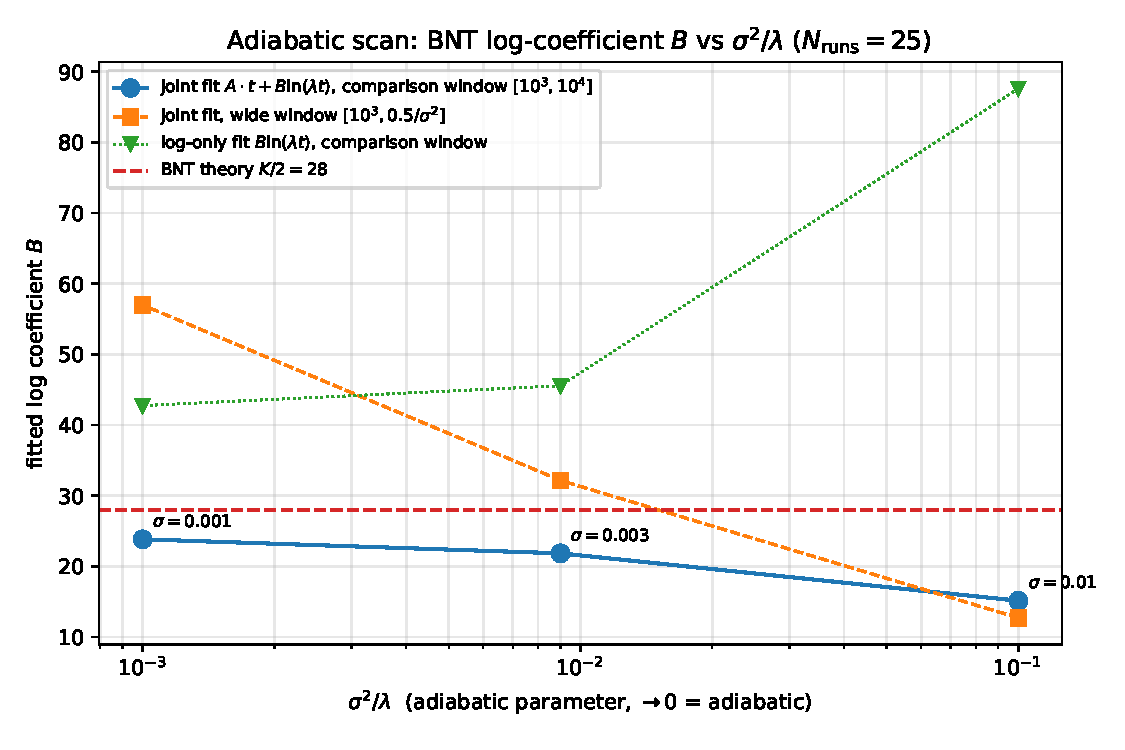
\includegraphics[width=0.85\linewidth]{figs/Fig6.pdf}\end{center}

 and 

\begin{center}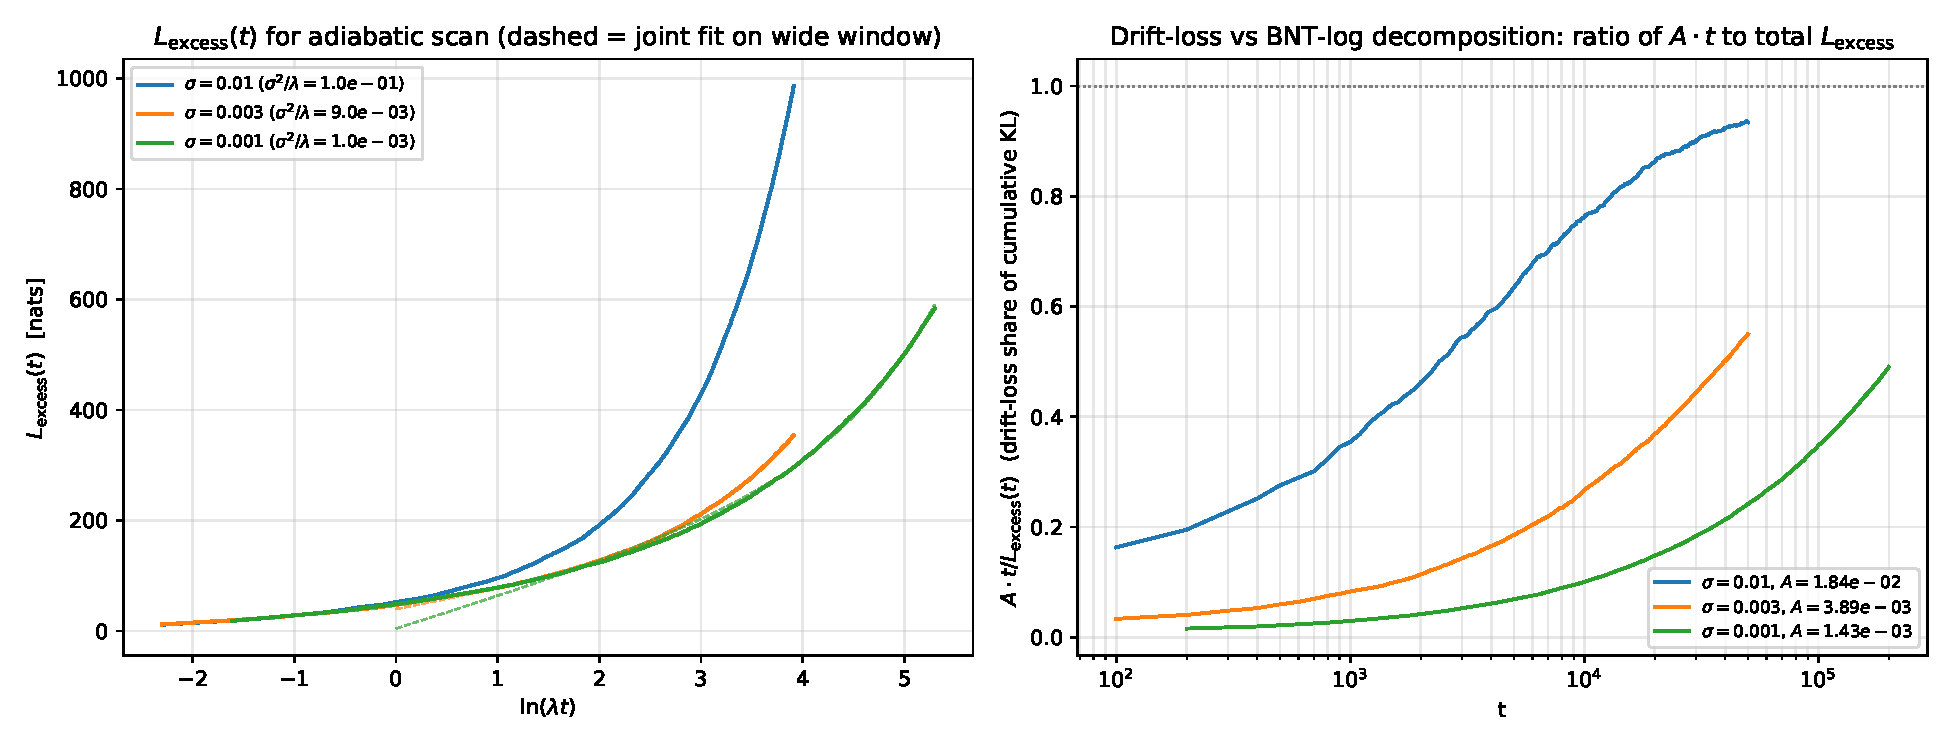
\includegraphics[width=0.85\linewidth]{figs/Fig7.pdf}\end{center}





\subsection*{S4.4 Reproducibility: dependencies and archiving}\label{s4.4-reproducibility-dependencies-and-archiving}



\emph{Seed and dependencies.} The global \(\text{SEED} = 20260524\) is set at the start of \texttt{main.py} of each script; per-run offsets ensure the independence of the realizations. Dependencies --- \texttt{numpy}, \texttt{scipy}, \texttt{scikit-learn} (KSG), \texttt{matplotlib}; the exact versions are in the \texttt{requirements.txt} of each directory.



\emph{Full set of commands.} From the repository root, sequentially \texttt{python\ simulations/markov\_drift\{,\_ou,\_ou\_iinf\_adiab\}/main.py}; the total runtime on a mid-range laptop is \(\sim 7\)--\(12\) minutes.



\emph{Zenodo archiving.} A versioned snapshot with a DOI is archived on Zenodo (DOI: 10.5281/zenodo.21039182, release \texttt{v1.0-submission}); reproduction is also possible by cloning \texttt{andriishin/landauer-nostalgia-oa} at the tag \texttt{v1.0-submission} (the same snapshot archived on Zenodo).



\begin{center}\rule{0.5\linewidth}{0.5pt}\end{center}



\section*{\texorpdfstring{S5. Full apparatus of § 5 main: Remarks 1--6 to Lemma 2, the protocol of § 5.2, \(\nu_c\) and \(\tau_{\text{reset}}^*\)}{S5. Full apparatus of § 5 main: Remarks 1--6 to Lemma 2, the protocol of § 5.2, \textbackslash nu\_c and \textbackslash tau\_\{\textbackslash text\{reset\}\}\^{}*}}\label{s5.-full-apparatus-of-5-main-remarks-16-to-lemma-2-the-protocol-of-5.2-nu_c-and-tau_textreset}



This section collects the formal details of § 5 main, moved here to unburden the main exposition. Structure: S5.1 --- the six Remarks to Lemma 2 (§ 4.4 main fixes the formulation (8a) and a brief statement; here --- their full unfolding); S5.2 --- item 5 of the protocol of § 5.2 main (the prohibition on revising the definition of the measured object) with a justification via (Wolpert 1996) no-free-lunch; S5.3 --- the balance condition for the existence of \(\nu_c\) via (11) and a discussion of its structural status; S5.4 --- the optimal \(\tau_{\text{reset}}^*\) (12), its relation to dynamic regret bounds (Besbes et al.~2015); S5.5 --- the analogy with spin glasses via (Hopfield 1982; Amit et al.~1985; Engel and Van den Broeck 2001).



\subsection*{S5.1 The six Remarks to Lemma 2}\label{s5.1-the-six-remarks-to-lemma-2}



\textbf{Remark 1 (stationary limit).} The stationary limit of Lemma 2 is given \emph{not} by \(\tau_E \to \infty\) (that passage violates the condition \(c < 1\) by \((*)\) main), but by formula (1) main at \(\dot{E}_{\text{store}} = \dot{E}_{\text{grow}} = 0\) (§ 2.2 main): in that regime the nostalgic bits carry no cost, and the scale \(\nu^{\text{theor}}\) via (7) main loses its thermodynamic meaning (the same for \(\nu^{\text{op}}\) at \(\hat P \to P_0\)). Thus Lemma 2 does not contradict the stationary result on memory drift (Andriishin 2026, § 2.1), but \emph{supplements} it with a new regime: at \(\dot E_{\text{store}} > 0\) or \(\dot E_{\text{grow}} > 0\) the condition (8a) is in force, while in the stationary limit it degenerates through the vanishing of both rates.



\textbf{Remark 2 (computability and falsifiability of \((*)\)).} The constant \(c\) from \((*)\) main is a \emph{computable} function of three measurable parameters \((\dot{M}_{\text{refresh}}, \tau_E, |M_{\le t}|)\), not a free parameter of the theory. Lemma 2 is applicable at measured \(c < 1\); at \(c \ge 1\) the system passes into a \emph{sliding-window} regime: over the interval \(\tau_E\) the entire memory is fully updated, there is no archival layer, and the non-stationary theory degenerates. The test on \(c\) is an empirical condition of applicability, separating systems with an archival layer from those without. An LLM with a long context and an \(M_t\) layer of order \(10^5\)--\(10^6\) tokens at inference gives \(\dot{M}_{\text{refresh}} \tau_E \gg |M_t|\), \(c \gg 1\), and Lemma 2 assigns it to the sliding-window regime --- the theory, by its own condition, removes this layer from its domain of applicability (§ 8.3 main).



\textbf{Remark 3 (substantiveness of (8a) beyond a definition).} The fraction \(1-c\) is arithmetic (the ratio of the number of non-updated bits to the full memory size), whereas \(\nu^{\text{theor}}\) by (7) main is information-theoretic (the normalized MI deficit). The substantive part of Lemma 2 is the proof that the MI contribution of a non-updated bit to \(I_{\text{pred}}(t,\tau)\) asymptotically vanishes by DPI through the decorrelation of the OU latent with characteristic time \(\tau_E\) (the latent covariance; the conditional MI by S1.5a decays twice as fast, with \(\tau_E/2\), since \(I \approx \tfrac{1}{2}\rho^2\); the detailed proof --- S1 supplementary via MI-tensorization over the independent OU coordinates, § S1.5). Three conditions are required: (i) decorrelation of the optimal statistic with \(\tau_E\); (ii) an ideal observer in the denominator of (7) main; (iii) FIFO refresh. If any of (i)--(iii) is violated, the inequality (8a) is not derivable from the arithmetic \(c\).



\textbf{Remark 4 (extension to the general non-stationary class).} The base Lemma 2 is proved for the OU parametrization of the logits (§ 5.2 main, S1--S2 supplementary). The PSP surrogate (§ 6.1 main) and multiscale drift reproduce the result \emph{illustratively} at \(\lambda \tau_{\text{relax}} \ll 1\) through a single decorrelation mechanism with an effective \(\tau_E\), but there is no rigorous proof for non-OU classes in the present work; see § 8.5 main, an open problem. The Wolpert no-free-lunch (Wolpert 1996) gives a fundamental justification for narrowing the class of § 5.2: a universal theory of non-stationary learnability without an a priori restriction of the class is impossible; the slow-driving class is a necessary narrowing, not a methodological choice.



\textbf{Remark 5 (per-bit-uniformity).} The passage from the arithmetic fraction of non-updated bits \(c\) to the information-theoretic inequality \(\nu^{\text{theor}} \ge 1 - c\) (on the prediction-shortfall scale, normalized by the environment optimum \(I_{\text{pred}}^{\text{opt}}\) --- precisely where the floor is substantive; on the ballast scale \(\nu^{\text{Still}} \to 1\) trivially) requires additivity of MI over the independently updated bits:



\[I(M^{\text{refr}}; X_E^{[t,t+\tau]}) \le c \cdot I_{\text{pred}}^{\text{opt}} \cdot (1+o(1)).\]



The normalization by \(I_{\text{pred}}^{\text{opt}}\) (rather than by \(I_{\text{mem}}\)) is essential: the floor asserts that the fraction refreshed within \(\tau_E\) captures no more than a fraction \(c\) of the \emph{optimally predictable} future of the environment. In the slow-driving limit the refresh fraction accumulates no cross-bit redundancy (Clarke and Barron 1990); the full proof for the OU parametrization is S2 supplementary. If the condition is violated, \(c \to \kappa c\), \(\kappa \ge 1\), and Lemma 2 is stated with a multiplicative correction \(\nu^{\text{theor}} \ge 1 - \kappa c\); in the OU class with independent \(W_{ij}\) and the diagonal anchor \(\theta_{ii} \equiv 0\) the prior is diagonalized by construction, whereas the posterior carries a within-row Fisher correction (S2.7), empirically \(\kappa \approx 1\) in the realizations of § 6.2 (an analytic closure at the realized parameters is an open problem, § 8.5 main).



\textbf{Remark 6 (softmax-regularity for OU).} The transfer of the OU decorrelation from the autocovariance of the logits \(\theta_v(t)\) to any bounded measurable functional \(\xi(\theta_v)\) (in particular, to the entries of the transition matrix \(P_{ij}(\theta_v)\) and to any sufficient prediction statistic) is ensured by the Lipschitz continuity of the softmax in total variation on the set of logits with finite stationary variance \(\sigma^2/(2\lambda)\). Via MI-tensorization over the independent OU coordinates (§ S1.5) and DPI, the exponential decay \(\mathbb{E}[\theta_v(t)\theta_v(s)] \propto e^{-(t-s)/\tau_E}\) is carried to the covariance of any bounded \(\xi\) with the same characteristic time \(\tau_E\); the conditional MI (S1.5a, S1.6), however, decays twice as fast --- with \(\tau_E/2\) (rate \(2/\tau_E\)), since \(I \approx \tfrac{1}{2}\rho^2\) at small correlation. The full proof --- S1 supplementary (five steps: Lipschitz softmax in \(\ell_\infty\); transfer to the TV of the transition matrix; boundedness of the OU trajectory on a ball \(R(\delta)\) with probability \(1-\delta\); transfer of the decay to the covariance of \(\xi\); translation of the TV bound into a bound on the conditional MI via \(\chi^2\) and DPI).



Lemma 2 in light of Remarks 1--6 is constructive: at \((*)\) it points to an explicit mechanism of the emergence of nostalgia (the desynchronization of the optimal feature through OU decorrelation) and a physical obstruction to its being zero (the finite memory-update rate under FIFO scheduling). The joint action of Remarks 5--6 is the structural justification of the claimed asymptotics \(\nu^{\text{theor}} \ge 1 - c\) on the prediction-shortfall scale in the OU class of § 5.2 main; Remark 2 fixes the domain of applicability through the measurable condition \(c < 1\).



\subsection*{S5.2 Protocol of § 5.2 main, item 5: prohibition on revising the definition of the measured object}\label{s5.2-protocol-of-5.2-main-item-5-prohibition-on-revising-the-definition-of-the-measured-object}



Item 5 of the protocol (§ 5.2 main) is a pre-registration commitment protecting falsifiability: the operational definition of the measured quantity is fixed \emph{before} the data and is not revised under the former name of the theory after the data arrive. Under a systematic discrepancy between prediction and measurement, two honest moves remain: (a) refute the theory; (b) explicitly change its name, leaving the old name with the original definition. The rule is symmetric --- it binds theorist and empiricist equally.



\emph{Why this is needed.} The standard response to the failure of an empirical test is either to reject the theory or to narrow the conditions of its applicability (add caveats); both moves are legitimate and keep the test strict. Item 5 closes only the third, methodologically dubious path --- revising the very \emph{operational definition} of the measured object while keeping the theory's name (the classic ad hoc rescue in Popper's sense, disguised as a technical refinement of the operationalization). The symmetry makes the discipline honest in both directions: the empiricist does not ``refine'' the definition of the measured quantity post hoc to make the data agree with the theory; the theorist does not ``refine'' the definition of the predicted quantity post hoc to make them disagree.



\emph{How this is enforced in the work.} The cumulative excess-loss \(L_{\text{excess}}(t)\) (S8.1) is retained in § S8 as a separate, explicitly labeled counterfactual diagnostic, and is not used as an operationally measurable \(I_{\text{pred}}\): \(L_{\text{excess}}\) requires access to the ground truth \(\theta_v(s)\), unavailable in real biological systems, so identifying it with the one-step MI (4) main under the name ``predictive information'' would be a post hoc revision of the measured object. The theoretical constructions (Lemma 2, \(\nu_c\), \(C_v^{\text{predictive}}\)) rely on \(\nu^{\text{theor}}\) by (7) main; the operational predictions (§ 8.6 main, P.1, P.2) rely on \(\nu^{\text{op}}\) by (7') main. Substitution under one name is excluded; separate bookkeeping of the two quantities is not.



\subsection*{\texorpdfstring{S5.3 Existence of \(\nu_c\): the balance condition (11) on the \(\nu^{\text{op}}\) scale}{S5.3 Existence of \textbackslash nu\_c: the balance condition (11) on the \textbackslash nu\^{}\{\textbackslash text\{op\}\} scale}}\label{s5.3-existence-of-nu_c-the-balance-condition-11-on-the-nutextop-scale}



The regime threshold \(\nu_c\) is defined on the \emph{prediction-shortfall} scale \(\nu^{\text{op}}/\nu^{\text{theor}}\) (normalized by the environment optimum \(I_{\text{opt}}\)) --- the very one on which the floor (8a) of Lemma 2 is substantive and which distinguishes the regimes in the figures of § 6 (the ballast scale \(\nu^{\text{Still}} \approx 1\) carries no threshold). The balance estimate from the condition of equality of the gain \(\dot{I}_{\text{pred}}\) and the losses from aging (formula (11) main):



\[\nu_c^{\text{theor}} \cdot |M_{\le t}| / \tau_{1/2} = (1 - \nu_c^{\text{theor}}) \cdot \dot{M}_{\text{refresh}}.\]



The dimensionless \(\eta_M := \dot{M}_{\text{refresh}} \tau_{1/2} / |M_{\le t}|\) formally gives \(\nu_c^{\text{theor}} = \eta_M / (1 + \eta_M)\). \emph{Explicit substitution (reproducible).} Take the working identification \(\tau_{1/2} \sim \tau_E = 1/\lambda = 10^3\) steps (the bit-accuracy half-life is set by the environment correlation time). (i) \emph{Reset regime} (FIFO window \(\tau_w\)): the whole window is refreshed within \(\tau_w\), so \(\dot M_{\text{refresh}} \approx |M_{\le t}|/\tau_w\) and \(\eta_M \approx \tau_{1/2}/\tau_w = \tau_E/\tau_w\). For \(\tau_w = \{100, 500, 2000\}\): \(\eta_M \approx \{10,\, 2,\, 0.5\}\), whence \(\nu_c^{\text{theor}} = \eta_M/(1+\eta_M) \approx \{0.91,\, 0.67,\, 0.33\}\) --- whereas the observed \(\langle\nu^{\text{op}}\rangle = \{0.382,\, 0.298,\, 0.600\}\) (§ 6.1 main): neither the numbers nor the monotonicity in \(\tau_w\) agree. (ii) \emph{Accumulation regime} (drift with no reset, \(\tau_w \to \infty\)): memory grows without bound, \(|M_{\le t}| \sim I_{\text{mem}} = (K/2)\ln t \approx 322\) nats at \(t = 10^5\), while the effective refresh decays, \(\dot M_{\text{refresh}} \sim K/t = 56/10^5\); then \(\eta_M \approx (K/t)\cdot\tau_E/|M_{\le t}| = (5.6\cdot10^{-4}\cdot10^3)/322 \approx 1.7\cdot10^{-3}\) and \(\nu_c^{\text{theor}} \approx 1.7\cdot10^{-3}\), whereas the observed \(\langle\nu^{\text{op}}\rangle \to 0.999\) --- a discrepancy of more than two orders of magnitude. Direct substitution of the simplest form of (11) thus yields numerical values inconsistent with the observed \(\nu^{\text{op}}\) scale of the PSP simulation of § 6.1 main, where \(\nu^{\text{op}}\) is bounded under reset (\(0.30\)--\(0.60\)) and goes to \(0.999\) under memory accumulation --- a discrepancy with the balance substitution of more than an order of magnitude.



\emph{Structural status of (11).} (11) is treated as a \emph{structural balance condition}, not a quantitative predictor: the work postulates the existence of \(\nu_c^{\text{theor}} \in (0, 1)\) as a fixed point of the balance between information gain and losses from aging on the prediction-shortfall scale. The discrepancy with the operational \(\nu^{\text{op}}\) scale supports this decision --- direct substitution of the simplest form of (11) is rejected, which is recorded as the boundary of its interpretive power. The derivation of a quantitative formula \(\nu_c^{\text{theor}}(\lambda, \sigma, K, \tau_{1/2}, \dot M_{\text{refresh}})\) is an open problem of § 8.5 main.



\emph{Active part of memory.} In (11), \(|M_{\le t}|\) is the \emph{active} part of memory, not the structural capacity limit \(|M_{\le t}^{\text{cap}}|\). In § 6.1 main the estimator model has \(K = k(k-1) = 56\) free off-diagonal parameters; in systems with expanding memory the active part grows over time, and the numerical value of \(\nu_c^{\text{theor}}\) is time-dependent. The operational threshold on the \(\nu^{\text{op}}\) scale is \(\nu_c^{\text{op}}\) by (7') main, not \(\nu_c^{\text{theor}}\); the working assumption of § 4.1 main about the stability of the regime threshold under a change of normalization provides the passage between them with a possible numerical shift.



\subsection*{\texorpdfstring{S5.4 The optimal \(\tau_{\text{reset}}^*\) and its relation to dynamic regret}{S5.4 The optimal \textbackslash tau\_\{\textbackslash text\{reset\}\}\^{}* and its relation to dynamic regret}}\label{s5.4-the-optimal-tau_textreset-and-its-relation-to-dynamic-regret}



The optimal \(\tau_{\text{reset}}^*\) maximizes the late-time predictive information \(\langle I_{\text{pred}}\rangle\) (equivalently --- minimizes the prediction shortfall \(\langle\nu^{\text{op}}\rangle\)): frequent resets discard still-useful memory, rare ones lead to nostalgic collapse (§ 5.3 main). The structural estimate:



\[\tau_{\text{reset}}^* \sim \tau_E \cdot \log(|M_{\le t}^{\text{cap}}|/\dot{M}_{\text{refresh}} \tau_E),\]



where \(|M_{\le t}^{\text{cap}}|\) is the structural memory-capacity limit. \emph{Derivation of the optimum (3--4 lines).} After a reset, freshly loaded memory predicts with a value that ages exponentially with age \(a\) (the environment drift desynchronizes the memory): the density of useful information is \(I(a) = I_0\,e^{-a/\tau_E}\). A reset/reload of capacity \(|M_{\le t}^{\text{cap}}|\) at refresh rate \(\dot M_{\text{refresh}}\) costs a dead time \(T_c = |M_{\le t}^{\text{cap}}|/\dot M_{\text{refresh}}\) (a linear cost for the refresh). The long-run-average useful information per cycle of length \(\tau_{\text{reset}}\):



\[\langle I\rangle(\tau_{\text{reset}}) = \frac{\int_0^{\tau_{\text{reset}}} I_0 e^{-a/\tau_E}\,da}{\tau_{\text{reset}} + T_c} = \frac{I_0\tau_E\,(1 - e^{-\tau_{\text{reset}}/\tau_E})}{\tau_{\text{reset}} + T_c}.\]



The condition \(d\langle I\rangle/d\tau_{\text{reset}} = 0\) gives the transcendental \(e^{\tau_{\text{reset}}/\tau_E} = 1 + \tau_{\text{reset}}/\tau_E + T_c/\tau_E\), whose solution at large \(T_c/\tau_E = |M_{\le t}^{\text{cap}}|/(\dot M_{\text{refresh}}\tau_E) \gg 1\) is \(\tau_{\text{reset}}^*/\tau_E \approx \ln(T_c/\tau_E)\), i.e.~the logarithmic form above. The logarithmic dependence is the standard form of the optimum for processes with exponential aging and a linear cost of updating.



\emph{Biological analogy.} The generation time of a taxon correlates with the rate of change of the econiche --- an empirical regularity of population biology, consistent with (12) main up to a logarithmic factor. In mammals, in early embryogenesis and the germline, an almost complete erasure of DNA methylation occurs with re-establishment (Reik 2007); this can be read as a mechanism of \(\tau_{\text{reset}}^*\) on the generational scale --- a periodic reset of the nostalgic layer for the sake of restoring \(\nu^{\text{op}} \to 0\) in the new generation.



\emph{Relation to dynamic regret bounds.} In non-stationary stochastic optimization (Besbes et al.~2015) (Theorem 2, stochastic setting) the regret-optimal length of a restart epoch has a \emph{power-law} structure: the optimal length \(\propto (T/V_T)^{2/3}\), where \(V_T\) is the variation of the target on the horizon \(T\). This differs from the logarithmic form \(\tau_{\text{reset}}^* \sim \tau_E \log(\cdot)\) of main § 8.4(b): the main text gives a \emph{logarithmic} form through a linear update cost with exponential aging, whereas the BGZ regret-optimal restart is a \emph{power law} \((T/V_T)^{2/3}\). Only the monotonicity in \(\tau_E\) agrees (slower drift --- rarer reset), not the functional form. Under no-free-lunch (Wolpert 1996) a universal \(\tau_{\text{reset}}^*\) is impossible, consistent with the conditionality of (12) main on the class of § 5.2 main.



\subsection*{S5.5 Analogy with spin glasses}\label{s5.5-analogy-with-spin-glasses}



\begin{enumerate}

\def\labelenumi{(\arabic{enumi})}

\setcounter{enumi}{10}

\tightlist

\item

  main is a mean-field balance, structurally analogous to replica symmetry in the statistical mechanics of learning (Engel and Van den Broeck 2001). In the classical Hopfield model (Hopfield 1982) the critical load \(\alpha_c \approx 0.138\) (Amit et al.~1985) is the threshold beyond which associative memory loses the ability to retrieve stored patterns without errors. Our \(\nu_c^{\text{theor}}\) is the analogue in a non-equilibrium learning system: the threshold beyond which the nostalgic fraction exceeds a critical share and the predictive power \(I_{\text{pred}}(t)\) (and with it \(\eta_v(t)\)) collapses.

\end{enumerate}



A quantitative link between \(\nu_c^{\text{theor}}\) and the Hopfield \(\alpha_c\) is a separate problem: \(\alpha_c\) is the ratio of the number of stored patterns to the number of neurons in an equilibrium system with a fixed set of targets, \(\nu_c^{\text{theor}}\) is the threshold ratio of the nostalgic fraction in a non-equilibrium system with a drifting latent parameter. The structural correspondence --- both quantities reflect the limiting load on memory capacity in systems with a fixed number of degrees of freedom; their dynamical characteristics, however, differ substantially.



\begin{center}\rule{0.5\linewidth}{0.5pt}\end{center}



\section*{S6. Full technical details of § 6 main: PSP parameters, the Robbins--Monro learner, the extended-window control}\label{s6.-full-technical-details-of-6-main-psp-parameters-the-robbinsmonro-learner-the-extended-window-control}



This section collects the technical details of the numerical illustrations of § 6.1 (PSP) and § 6.2 (OU) main, which in the main text are left as a brief statement of results with a cross-reference here. Structure: S6.1 --- the full parameters of the PSP simulation (§ 6.1 main) and the MI estimator; S6.2 --- the simulation pseudocode and comparative analysis of estimators; S6.3 --- the Robbins--Monro online learner of the OU simulation (§ 6.2 main) and its asymptotic Bayes-optimality; S6.4 --- the numerical estimate of \(c\) for Robbins--Monro and the discrepancy with the prediction (8a); S6.5 --- the extended-window negative control of the adiabatic scan and the \(C_v^{\text{static}}/C_v^{\text{predictive}}\) divergence; S6.6 --- the empirical \(\nu_c^{\text{op}}\) and its status.



All reproducibility parameters (seed, library versions, directories) are in S4 supplementary (simulation parameters for reproducibility); this section focuses on the methodological justification of the parameter choices and the interpretation of the results.



\subsection*{S6.1 PSP simulation (§ 6.1 main): full parameters and estimator}\label{s6.1-psp-simulation-6.1-main-full-parameters-and-estimator}



\emph{Model.} A finite-state Markov process with Poisson switches of the transition matrix. Alphabet \(\Omega = \{1, \ldots, k\}\), \(k = 8\). The matrix \(P(t)\) is piecewise-constant on the intervals \([T_i, T_{i+1})\); the switching times \(\{T_i\}\) form a Poisson stream with intensity \(\lambda\). At the moment \(T_i\) the matrix is updated to a random stochastic \(P^{(i)} \sim \text{Dirichlet}(\alpha = 0.3)\) by rows. \(\alpha = 0.3\) gives \(\langle \tau_{\text{relax}} \rangle \approx 2\)--\(3\) steps and \(\lambda \tau_{\text{relax}} \approx 3 \cdot 10^{-3} \ll 1\) with margin --- slow-driving is satisfied.



\emph{Observer memory.} The observer system holds a memory \(M_t\) consisting of an estimate of the current transition matrix \(\hat{P}(t)\) over a sliding window of length \(\tau_w\) with Laplace smoothing (a pseudocount of 1 per cell). The structural dimension of the model is \(K = k(k-1) = 56\) free off-diagonal parameters of the transition matrix (each row has \(k-1\) free cells). The efficiency denominator is the \emph{information} of the memory: \(I_{\text{mem}}(t) = (K/2)\ln(\max(N_{\text{obs}}, e))\) nats, where \(N_{\text{obs}}\) is the number of transitions held in memory (window fill \(\min(t, \tau_w)\)). This is the Bayesian stochastic complexity of a \(K\)-parameter model over \(N\) observations; by DPI \(I_{\text{pred}} \le I_{\text{mem}}\), and \(\eta_v = I_{\text{pred}}/I_{\text{mem}} \in [0,1]\) unconditionally.



\emph{Parameters of the three regimes.} Stationary regime: \(\lambda = 0\) (the matrix does not change), \(\tau_w \to \infty\), \(T_{\text{total}} = 10^4\) steps, averaging over 80 realizations. Drift, no reset: \(\lambda = 10^{-3}\) (mean \(\tau_E = 10^3\) steps between switches), \(\tau_w \to \infty\) (memory is not cleared, \(\hat{P}(t)\) is averaged over the whole history), \(T_{\text{total}} = 10^5\) steps, 60 realizations. Drift with reset: \(\lambda = 10^{-3}\), \(\tau_w \in \{100, 500, 2000\}\), \(T_{\text{total}} = 10^5\), 60 realizations.



\emph{Grid of \(\tau_w\) for Fig. 2.} Eight points \(\tau_w \in \{50, 100, 200, 500, 10^3, 2\cdot 10^3, 5\cdot 10^3, 10^4\}\) at \(\lambda = 10^{-3}\), \(T_{\text{total}} = 5 \cdot 10^4\), 40 realizations per point.



\subsection*{S6.2 Simulation pseudocode and comparative analysis of MI estimators}\label{s6.2-simulation-pseudocode-and-comparative-analysis-of-mi-estimators}



\emph{PSP simulation pseudocode.}



\begingroup\footnotesize\linespread{1}\selectfont
\begin{Verbatim}[breaklines=true]

for each condition (λ, τ_w):

    initialize P_0, draw T_1 ~ Exp(λ)

    initialize memory: counts = zero matrix (k × k); FIFO buffer of length τ_w

    for t = 1, 2, ..., T:

        if t >= T_i: update P to a random P^(i) ~ Dirichlet(α=0.3, k rows),

                     draw T_{i+1}

        X_t = sample from P_t[X_{t-1}, :]

        # sliding window: when the buffer is full, evict the oldest transition

        if τ_w < ∞ and buffer full: counts[evicted transition] -= 1

        counts[X_{t-1}, X_t] += 1; buffer <- (X_{t-1}, X_t)

        if t mod measure_every == 0:

            P_hat(t) = (counts + Laplace) normalized by rows

            N_obs(t) = counts.sum()                      # = min(t, τ_w)

            I_mem(t) = (K/2) ln(max(N_obs, e))           # K = k(k-1) = 56

            I_pred(t, τ) = I_opt(P_t,τ) - E_{x~π}[KL(P_t^τ(.|x) || P_hat^τ(.|x))], clipped below at 0

            I_pred(t, τ) = min(I_pred, I_mem)            # finite-sample guard (not the DPI theorem, § 3.1)

            η(t)        = I_pred(t, τ) / I_mem(t)

            ν_op(t)     = 1 - I_pred(t, τ) / I_opt(P_t, τ)   # leading nostalgia

            ν_Still(t)  = 1 - η(t)                            # ballast (secondary)

for each set (λ, τ_w): plot I_pred(t), ν_op(t), ν_Still(t)

\end{Verbatim}
\endgroup



\emph{MI estimator: KL-detuned proxy.} At a prediction horizon \(\tau\) the numerical estimate of the kernel definition (4) main is carried out via



\[\widehat I_{\text{pred}}(t, \tau) = I_{\text{opt}}(P(t), \tau) - \mathbb{E}_{X_t \sim \pi(t)}\!\bigl[ D_{\text{KL}}\!\bigl(P(t)^\tau(\cdot \mid X_t)\,\|\,\hat{P}(t)^\tau(\cdot \mid X_t)\bigr) \bigr],\]



clipped below at zero. Here \(I_{\text{opt}}(P, \tau) = H(\pi) - \sum_i \pi_i H(P^\tau_{i,\cdot})\) is the predictive information of the optimal observer with an exact model; a KL penalty for the mismatch of \(\hat{P}\) to the true \(P\) is subtracted. \emph{Relation to (4) main: the inequality linking the KL penalty to the conditional MI.} Rewrite the proxy in cross-entropy form. Expanding \(D_{\text{KL}}(P^\tau\|\hat P^\tau) = H_\times(P^\tau,\hat P^\tau) - H(P^\tau)\) (cross-entropy minus entropy) and substituting \(I_{\text{opt}} = H(\pi_{t+\tau}) - \mathbb{E}_i[H(P^\tau_{i,\cdot})]\):



\[\widehat I_{\text{pred}}(t,\tau) = H(\pi_{t+\tau}) - \mathbb{E}_{i\sim\pi}\bigl[H_\times(P^\tau_{i,\cdot}, \hat P^\tau_{i,\cdot})\bigr].\]



Now let \(I(X_t;X_{t+\tau}\mid\hat P(t)) = I_{\text{opt}} - \Delta\), where \(\Delta \ge 0\) is the \emph{actual} loss of predictive MI due to the substitution \(P \to \hat P\) (the reduction of the dependence between \(X_t\) and \(X_{t+\tau}\) visible through the model \(\hat P\)). The key step: this loss is majorized by the KL mismatch,



\[\Delta \;\le\; \mathbb{E}_{i\sim\pi}\bigl[D_{\text{KL}}(P^\tau_{i,\cdot}\|\hat P^\tau_{i,\cdot})\bigr],\]



since the KL ``overestimates'' the loss: it penalizes the full distributional discrepancy of \(P^\tau\) and \(\hat P^\tau\), whereas the MI decrement sees only that part of it which reduces the predictive dependence (Pinsker/DPI domination --- the MI decrement is bounded by the model divergence). Consequently



\[\widehat I_{\text{pred}}(t,\tau) = I_{\text{opt}} - \mathbb{E}_i[D_{\text{KL}}] \;\le\; I_{\text{opt}} - \Delta = I(X_t; X_{t+\tau}\mid\hat P(t)),\]



i.e.~the proxy is majorized from above by the conditional MI; the clipping below at zero is ensured by the non-negativity of the conditional MI. On the ergodic plateau \(\hat P(t) \to P(t)\) the KL penalty vanishes (\(\Delta \to 0\)), and \(\widehat I_{\text{pred}} \to I_{\text{opt}} = I(X_t; X_{t+\tau}\mid P_0)\), consistent with (4) main in the stationary limit.



\emph{Exact MI computation.} The mutual information in the Markov model is computed \textbf{exactly} from the transition structure (closed form), without a sampling estimator, so the observed qualitative patterns (Figs. 1--3 main) do not depend on the MI estimation method. Sampling estimators --- the discrete plug-in with bias correction (Treves and Panzeri 1995) and the continuous KSG estimator with \(k\)-NN, \(k_{NN} = 3\) (Kraskov et al.~2004) --- are intended for data from real systems (§ 3).



\emph{Dome-shaped dependence \(\langle I_{\text{pred}}\rangle(\tau_w)\).} The diagnostically leading curve of Fig. 2 main --- \(\langle I_{\text{pred}}\rangle\) as a function of \(\tau_w\) --- is dome-shaped with a maximum \(\langle I_{\text{pred}}\rangle^* = 0.467 \pm 0.006\) nats at \(\tau_w^* \approx 200\) steps; this is the non-stationary analogue of the bias--variance tradeoff of classical learning theory: a small \(\tau_w\) --- high variance of the estimator \(\hat P\) (too little data), a large \(\tau_w\) --- bias from averaging over no-longer-relevant regimes; the optimum \(\tau_w^*\) is a balance, analogous to structural risk minimization. The secondary axis \(\langle\eta_v\rangle = \langle I_{\text{pred}}/I_{\text{mem}}\rangle\) is structurally small (\(\langle\eta_v\rangle^* \approx 3.2 \cdot 10^{-3}\)) and its own optimum in \(\tau_w\) is shifted to \(\approx 100\) (a shorter window gives a smaller \(I_{\text{mem}}\), hence a larger \(\eta_v\)); this is a diagnostic of the ballast, not of prediction quality, so the leading curve is \(\langle I_{\text{pred}}\rangle\), not \(\langle\eta_v\rangle\).



The position of the maximum \(\tau_w^* \approx 0.2\,\tau_E < \tau_E = 1000\) is consistent with (12) main up to a logarithmic factor; the exact value of the optimum depends on fine estimator parameters (Laplace smoothing, the Dirichlet \(\alpha\)).



\subsection*{S6.3 The Robbins--Monro online learner of the OU simulation (§ 6.2 main)}\label{s6.3-the-robbinsmonro-online-learner-of-the-ou-simulation-6.2-main}



\emph{Maintaining the online estimate.} In the OU simulation (§ 6.2 main) the learner maintains an online estimate \(\hat\theta_v(t)\) via maximization of the conditional log-likelihood with a decaying step-size \(\eta_t = c_0/\sqrt{t}\) (\(c_0 = 3\)): at each step, on observing \((x_t \to x_{t+1})\),



\[\hat\theta_{x_t,j}(t+1) = \hat\theta_{x_t,j}(t) + \eta_t \cdot \bigl[\mathbb{1}[x_{t+1} = j] - \hat P_{x_t,j}(t)\bigr]\]



for \(j \ne x_t\). This is a diffusion-prior-Bayes approximation to the Bayesian update over the OU latent in the sense of § 5.2 main; the rate \(1/\sqrt{t}\) corresponds to the concentration of the posterior along each of the \(K\) directions and is asymptotically Bayes-optimal for regular parametric models (Clarke and Barron 1990, § 3).



\emph{Polyak--Ruppert averaging note.} The standard improvement of Robbins--Monro --- Polyak--Ruppert averaging of the iterates --- gives an asymptotically efficient estimate with smaller variance; it is not used in the present implementation, since the observed qualitative patterns (Figs. 4--5 main) are robust to the choice of Robbins--Monro variant up to log-factors on the final variance. Using Polyak--Ruppert would change the quantitative values of \(\eta_v(t)\) by a constant factor, but not the qualitative picture of the collapse.



\emph{Structural equivalence to Bayes.} Robbins--Monro with the stated rate \(\eta_t \propto 1/\sqrt{t}\) is structurally equivalent to the online approximation of the Bayesian update over the OU latent of § 5.2 main in the following sense: the post-cumulative distribution of the estimates \(\hat\theta_v(t)\) as \(t \to \infty\) concentrates around the conditional posterior mean with covariance of order \(\mathcal{F}^{-1}/t\), where \(\mathcal{F}\) is the Fisher information matrix of the parametric model (Clarke and Barron 1990). This is the justification for choosing \(\eta_t \propto 1/\sqrt{t}\) as functionally equivalent to a Bayesian learner \textbf{in the stationary case}.



\emph{Breakdown of Bayes-optimality under drift and the second learner.} The same asymptotic Bayes-optimality of Robbins--Monro is the \emph{cause} of its breakdown under a non-stationary target: the decay of the step \(\eta_t \to 0\) means that after some \(t\) the update is weaker than the OU-latent drift accumulated over a step, and the estimate \textbf{freezes} relative to the moving \(\theta_v(t)\). Therefore § 6.2 main compares Robbins--Monro with a second learner --- a \textbf{constant step} \(\eta_t = s\) (operating point \(s = 0.3\)). Both run on one trajectory and see the same transition; only the step-size schedule differs. The constant step does not freeze: it tracks the drift indefinitely, paying a residual floor of lag/noise of order \(\sim s\sigma^2/(2\lambda)\) per coordinate instead of going to \(\nu^{\text{op}} \to 1\). The operating point \(s = 0.3\) is chosen from the sweep of Fig. 5 (validated as near the interior optimum \(s^\star \approx 0.6\) at \(\sigma = 0.1\)): a small step under-tracks (lag), a large one overfits the OU noise. This contrast is a \emph{design lesson}, not a no-go: under non-stationarity the optimal estimator is not the asymptotically-optimal stationary one.



\subsection*{\texorpdfstring{S6.4 Numerical estimate of \(c\) for both learners and the floor (8a) on the \(\nu^{\text{op}}\) scale}{S6.4 Numerical estimate of c for both learners and the floor (8a) on the \textbackslash nu\^{}\{\textbackslash text\{op\}\} scale}}\label{s6.4-numerical-estimate-of-c-for-both-learners-and-the-floor-8a-on-the-nutextop-scale}



\emph{The floor is placed on the prediction-shortfall scale.} The floor (8a) of Lemma 2 --- \(\liminf \nu^{\text{theor}}(t) \ge 1 - c\) --- is substantive precisely on the \emph{prediction-shortfall} scale \(\nu^{\text{theor}}/\nu^{\text{op}}\) (normalized by the environment optimum \(I_{\text{opt}}\)): it says that no more than a fraction \(c\) of the optimally predictable future is extracted from memory refreshed within the environment correlation interval. On the ballast scale \(\nu^{\text{Still}} = 1 - I_{\text{pred}}/I_{\text{mem}}\) the corresponding inequality is trivial (\(\nu^{\text{Still}} \to 1\) structurally for a memory-accumulating system) and does not distinguish the regime. In the simulations of § 6.2, where the true value is known by construction, \(\nu^{\text{theor}} = \nu^{\text{op}}\), and the numerical check of (8a) proceeds on this scale.



\emph{Robbins--Monro --- the freezing limit \(c \to 0\).} The decaying step \(\eta_t = c_0/\sqrt t\) gives a vanishing effective refresh rate \(\dot M_{\text{refresh}}^{\text{eff}}(t) \sim K c_0/(\tau_E\sqrt t)\), i.e.~\(c(t) = \dot M_{\text{refresh}}^{\text{eff}}\,\tau_E/|M_{\le t}| \approx K c_0/(|M_{\le t}|\sqrt t) \to 0\) as \(t \to \infty\) (\(|M_{\le t}| = K\)). Correspondingly the floor \(1 - c \to 1\), and the \(\nu^{\text{op}}\) of the frozen RM grows monotonically toward one: the observed \(\nu^{\text{op}}(t) = 0.567 \to 0.747 \to 0.892\) (\(t = 2200, 10200, 20000\)), the late-time \(0.821 \pm 0.005\) --- qualitatively consistent with \(\nu^{\text{op}} \to 1\) at \(c \to 0\). The finiteness of the horizon (\(t \le 2\cdot10^4\)) and the approximateness of the per-bit-uniformity of Remark 5 (softmax nonlinearity, Remark 6) explain why the observed \(0.82\) has not yet reached one.



\emph{Constant step --- finite \(c\), finite floor.} The constant step \(\eta_t = s\) holds a nonzero refresh rate, \(c\) is finite and large, so the floor \(1 - c\) is finite and low: the observed \(\nu^{\text{op}} \approx 0.316 \pm 0.003\) (tracking floor \(0.283 \to 0.305 \to 0.331\), does \emph{not} grow). This is a direct illustration of the structure of Lemma 2: the floor \(1 - c\) is lower the higher the refresh rate relative to \(\tau_E\). A quantitative check of \(1-c\) as a \emph{pointwise} prediction on a concrete OU parametrization with a controlled \(\tau_E\) is an open problem of § 8.5 main (an explicit derivation of \(c\) from \((\sigma, \lambda, s)\) and the convergence of the per-bit-uniformity coefficient are required).



\subsection*{\texorpdfstring{S6.5 The extended-window negative control and the \(C_v^{\text{static}}/C_v^{\text{predictive}}\) divergence}{S6.5 The extended-window negative control and the C\_v\^{}\{\textbackslash text\{static\}\}/C\_v\^{}\{\textbackslash text\{predictive\}\} divergence}}\label{s6.5-the-extended-window-negative-control-and-the-c_vtextstaticc_vtextpredictive-divergence}



\emph{Negative control with an extended window.} Extending the window of the joint fit of the adiabatic scan (§ S8.3) to \([10^3, T_{\text{total}}]\) (instead of the fixed \([10^3, 10^4]\)) degenerates the fit: at \(\sigma^2/\lambda = 10^{-3}\) and \(T_{\text{total}} = 2\cdot 10^5\) the coefficient \(B/(K/2)\) grows to 2.0 --- an artifact of the Robbins--Monro \(1/\sqrt t\) bias of the learner on long horizons, not part of the BNT effect. The window \([10^3, 10^4]\) is chosen for direct comparison across the points of the adiabatic series and is consistent with the transient condition \(t \ll 1/\sigma^2\). This control pins the sensitivity of the result to the choice of fit window and prevents interpreting the monotone trend of \(B/(K/2)\) as the product of selective presentation.



\emph{Numerical scan \(B/(K/2) \in \{0.54, 0.78, 0.85\}\).} Full results --- § S8.3 (table of \(B\), \(B/(K/2)\), \(R^2\), drift-share); S4.3 supplementary (scan parameters).



\emph{The \(C_v^{\text{static}}/C_v^{\text{predictive}}\) divergence.} In the ``drift, no reset'' regime (§ 6.1 main), at \(\nu^{\text{op}}(t) \to 0.999\) we have \(C_v^{\text{predictive}}(t) = (1 - \nu^{\text{op}}(t)) \cdot C_v^{\text{static}}(t) \to 0\) (in (9) main it is \(\nu^{\text{theor}}\); in the simulations of § 6 \(\nu^{\text{op}} = \nu^{\text{theor}}\)), whereas \(C_v^{\text{static}}\) remains bounded below by the size of the accumulated memory \(\hat P(t)\). The ratio \(C_v^{\text{static}}/C_v^{\text{predictive}} \to \infty\) is a numerical illustration of the diagnostic signal of nostalgia (§ 4.3 main): two proxies that agree in the stationary regime diverge under observed drift. This operationalizes Prediction 1 of § 8.6 main: the crossing of \(\nu_c^{\text{op}}\) is diagnosed through the divergence of the two proxies, without direct measurement of \(\nu^{\text{op}}(t)\).



\subsection*{\texorpdfstring{S6.6 The empirical \(\nu_c^{\text{op}}\) and its status}{S6.6 The empirical \textbackslash nu\_c\^{}\{\textbackslash text\{op\}\} and its status}}\label{s6.6-the-empirical-nu_ctextop-and-its-status}



The empirical regime threshold is formulated on the \emph{operational} prediction-shortfall scale \(\nu^{\text{op}} = 1 - I_{\text{pred}}/I_{\text{opt}}\) --- the very one that distinguishes the regimes in the figures of § 6.1 (the ballast scale \(\nu^{\text{Still}} \approx 1\) does not distinguish the regime). In the validated PSP simulation \(\nu^{\text{op}}\) takes bounded values in the reset regimes (\(\langle\nu^{\text{op}}\rangle = 0.382 / 0.298 / 0.600\) at \(\tau_w = 100 / 500 / 2000\); the minimum at the optimal window \(\tau_w^* \approx 200\)) and goes to \(\langle\nu^{\text{op}}\rangle = 0.999\) in the collapse regime (drift, no reset). The threshold \(\nu_c^{\text{op}}\) thus lies \emph{between} the minimum over \(\tau_w\) (\(\approx 0.30\), adaptive regime) and one (collapse): it separates windows at which forgetting still saves prediction, from memory accumulation in which prediction is useless.



\emph{Honest caveat on the numerical value.} In the collapse regime the efficiency \(\eta_v = I_{\text{pred}}/I_{\text{mem}}\) is monotone (there is no peak), so the half-life moment of \(\eta_v\) is undefined and the definition ``half-life of \(\eta_v\)'' is inapplicable; a single universal number \(\nu_c^{\text{op}}\) is not extracted from the validated runs, and it is \textbf{not postulated} here. The structural statement of § 5.3 main about the existence of \(\nu_c \in (0,1)\) separating the adaptive regime and collapse is supported by the data (\(\nu^{\text{op}}\) is bounded under reset, \(\to 1\) under accumulation), but the concrete threshold number depends on the operational definition and the parameters of the PSP surrogate.



\emph{Discrepancy with (11).} The direct balance substitution \(\nu_c^{\text{theor}} = \eta_M/(1+\eta_M)\) in the simplest form of (11) main gives values inconsistent with the observed \(\nu^{\text{op}}\) scale of the PSP. Explicitly (full arithmetic --- S5.3 supplementary, working identification \(\tau_{1/2}\sim\tau_E=10^3\)): in the accumulation regime \(\eta_M \approx (K/t)\,\tau_E/|M_{\le t}| \approx 1.7\cdot10^{-3}\) gives \(\nu_c^{\text{theor}} \approx 1.7\cdot10^{-3}\) against the observed \(\langle\nu^{\text{op}}\rangle\to 0.999\) (a discrepancy of \(>2\) orders); in the reset regime \(\eta_M \approx \tau_E/\tau_w = \{10, 2, 0.5\}\) gives \(\nu_c^{\text{theor}} \approx \{0.91, 0.67, 0.33\}\) against \(\langle\nu^{\text{op}}\rangle = \{0.382, 0.298, 0.600\}\) --- a mismatch of numbers and monotonicity. This supports the decision of § 5.3 main / S5.3 supplementary to treat (11) as a structural balance condition, not a quantitative predictor. The derivation of a universal formula \(\nu_c^{\text{theor}}(\lambda, \sigma, K, \tau_{1/2}, \dot M_{\text{refresh}})\) is an open problem of § 8.5 main.



\emph{Stability under a change of normalization.} By DPI \(\nu^{\text{op}}(t) \le \nu^{\text{theor}}(t)\) pointwise (§ 4.1 main; a smaller denominator \(\hat E \le I_{\text{pred}}^{\text{opt}}\) in (7') gives a larger fraction and a smaller nostalgia); therefore the empirical threshold on the \(\nu^{\text{op}}\) scale is \(\nu_c^{\text{op}}\), a lower estimate for \(\nu_c^{\text{theor}}\). The working assumption of § 4.1 main about the monotonicity of the regime threshold under a change of normalization provides the applicability of the operational \(\nu_c^{\text{op}}\) as a surrogate for the theoretical \(\nu_c^{\text{theor}}\) with a possible numerical shift, but without a qualitative displacement of the threshold.



\begin{center}\rule{0.5\linewidth}{0.5pt}\end{center}



\section*{\texorpdfstring{S7. Active inference: full formal correspondence between \(\eta_v\) and EFE, \(\rho(t)\), caveats}{S7. Active inference: full formal correspondence between \textbackslash eta\_v and EFE, \textbackslash rho(t), caveats}}\label{s7.-active-inference-full-formal-correspondence-between-eta_v-and-efe-rhot-caveats}



This section collects the formal details of § 7 main, moved here to unburden the main exposition. Structure: S7.1 --- the heuristic correspondence \(\Delta G^{\text{epist}}\) ↔ \(-\Delta I_{\text{pred}}\) (S7.1), with a full justification and unit conversion; S7.2 --- the conjecture (S7.2) with its explicit conjectural status and a discussion of the direction of formalization; S7.3 --- the categorical caveat \(I_q(s'; o') \ne I(X_t; X_{t+\tau})\) via the sufficiency of \(\hat P(t)\); S7.4 --- the context of sophisticated inference (Friston et al.~2021) and the Pearl/Friston-blanket (Bruineberg et al.~2018; Bruineberg et al.~2022) demarcation; S7.5 --- the rebuttal of Andrews (2021) / Williams (2020) via a cross-reference to paper \#1; S7.6 --- the informational rejuvenation metric \(\rho(t)\) in detail, with its empirical interpretation.



\subsection*{S7.1 Heuristic correspondence: full justification}\label{s7.1-heuristic-correspondence-full-justification}



In the active-inference formulation (Friston et al.~2017a, eq. 3; Parr et al.~2022, ch.~7) the expected free energy of a policy \(\pi\) is measured in nats and is



\[G[\pi] = \mathbb{E}_{q(o', s' \mid \pi)}\!\left[\ln q(s' \mid \pi) - \ln p(o', s'\mid C)\right],\]



where \(p(o', s'\mid C)\) is the preference distribution with parameter \(C\) encoding the agent's goals. \emph{Derivation of the decomposition (reproducing Friston et al.~2017a, one line of algebra).} Factorizing \(p(o', s'\mid C) = p(o'\mid C)\,q(s'\mid o',\pi)\) (preferences over observations, the posterior over states approximates \(q(s'\mid o',\pi)\)) and substituting,



\[G = \mathbb{E}_q\bigl[\ln q(s'\mid\pi) - \ln q(s'\mid o',\pi)\bigr] - \mathbb{E}_q[\ln p(o'\mid C)] = -\mathbb{E}_{q(o'\mid\pi)}\bigl[D_{\text{KL}}(q(s'\mid o',\pi)\|q(s'\mid\pi))\bigr] - \mathbb{E}_q[\ln p(o'\mid C)],\]



where the first term collapsed into the (negative) expected KL divergence posterior↔prior over states. In total \(G = -\mathbb{E}_q[D_{\text{KL}}(q(s'\mid o',\pi)\|q(s'\mid\pi))] - \mathbb{E}_q[\ln p(o'\mid C)]\): epistemic value (information gain about hidden states; the minus sign --- minimizing \(G\) maximizes it) plus pragmatic value (closeness to preferences).



\emph{Unit conversion.} Both \(G\) and \(I_{\text{pred}}\) are measured in \textbf{nats} (Appendix A main). Conversion to energy units via \(\beta_v = 1/(k_B T)\) gives \(E_G = k_B T \cdot G_{\text{[nats]}}\) and, similarly, \(E_{I_{\text{pred}}} = k_B T \cdot (I_{\text{pred}})_{\text{[nats]}}\). For the increment over a policy window \(\Delta t\):



\begin{equation}k_B T \cdot \Delta G^{\text{epist}}[\pi]\bigr|_{\Delta t} \approx -k_B T \cdot \Delta I_{\text{pred}}\bigr|_{\Delta t}, \tag{S7.1}\end{equation}



up to an additive constant that absorbs the pragmatic contribution and is independent of \(\pi\). Both sides have the dimension of energy (J); the minus sign reflects the convention ``\(G\) is minimized when \(\dot{I}_{\text{pred}}\) is maximized''; the equivalent dimensionless form is obtained by dividing by \(k_B T\).



\emph{Conjectural status.} (S7.1) is fixed as a \emph{heuristic correspondence}, not as a proved inequality. Proof of a rigorous inequality requires (i) careful treatment of the time derivatives in a non-stationary generative model; (ii) a demonstration that the pragmatic contribution is indeed independent of \(\pi\) on the time scale \(\Delta t\); (iii) accounting for the corrections from the categorical caveat S7.3. All three ingredients are absent in the existing literature on active inference in the non-stationary regime.



\subsection*{S7.2 Conjecture: conjectural status}\label{s7.2-conjecture-conjectural-status}



The conjectural theorem --- the direction in which (S7.1) can be turned into a rigorous inequality:



\begin{equation}k_B T \cdot \Delta G^{\text{epist}}[\pi]\bigr|_{\Delta t} \stackrel{\text{conj.}}{\ge} -k_B T \cdot \Delta I_{\text{pred}}\bigr|_{\Delta t}, \tag{S7.2}\end{equation}



where the label ``conj.'' marks the conjectural status. Formal provability of (S7.2) is an open problem, requiring careful treatment of the time derivatives and a non-stationary generative model in an extended active-inference framework (Parr et al.~2022).



\emph{Sophisticated inference as a direction of formalization.} Sophisticated inference (Friston et al.~2021) extends standard active inference to policies that account for post-observational updates of future prior distributions; this is a natural frame for careful treatment of the time derivatives in a non-stationary generative model. A proof of (S7.2) in the sophisticated-inference framework is a natural next step of the extension of the present work.



\subsection*{\texorpdfstring{S7.3 Categorical caveat \(I_q(s'; o') \ne I(X_t; X_{t+\tau})\)}{S7.3 Categorical caveat I\_q(s\textquotesingle; o\textquotesingle) \textbackslash ne I(X\_t; X\_\{t+\textbackslash tau\})}}\label{s7.3-categorical-caveat-i_qs-o-ne-ix_t-x_ttau}



The epistemic value in (Friston et al.~2017a) is the mutual information \(I_q(s'; o'\mid\pi)\) between the hidden state \(s'\) and the observation \(o'\), whereas \(I_{\text{pred}}(t,\tau)\) by (4) main is the MI between two successive observations \(X_t\) and \(X_{t+\tau}\). These are categorically distinct objects: the first is the MI at a single time point between latent and observation, the second is the MI between two time moments along the observed trajectory.



\emph{Bridge via the sufficiency of \(\hat P(t)\).} Under the interpretation \(s' = \theta_v(t+\tau)\), \(o' = X_{t+\tau}\) and the condition \(X_{t+\tau} \perp \theta_v(t) \mid \hat P(t)\) (statistical sufficiency of \(\hat P(t)\): the current estimate screens the stale latent from the future observation), the bridge is derived via the chain rule for MI and DPI. Condition on \(\hat P(t)\). The generative model makes \(X_{t+\tau}\) depend on the past --- in particular on \(X_t\) --- \emph{only} through the current latent \(\theta_v(t+\tau)\), which sets the transition structure; this is a Markov chain



\[X_t \;\to\; \theta_v(t+\tau) \;\to\; X_{t+\tau} \quad (\text{given } \hat P(t)).\]



By the data-processing inequality on this chain (Cover and Thomas 2006, ch.~2.8) the conditional MI does not increase under coarse-graining \(\theta_v(t+\tau) \to X_t\):



\[I_{\text{pred}}(t,\tau) = I\bigl(X_t; X_{t+\tau}\mid\hat P(t)\bigr) \;\le\; I\bigl(\theta_v(t+\tau); X_{t+\tau}\mid\hat P(t)\bigr) = I_q\bigl(\theta_v(t+\tau); X_{t+\tau} \mid \hat P(t)\bigr).\]



The sufficiency of \(\hat P(t)\) guarantees that the only channel of latent connection with \(X_{t+\tau}\) is through \(\theta_v(t+\tau)\) (the stale \(\theta_v(t)\) is screened), so the chain is closed and DPI applies. The right-hand side is the epistemic value (S7.1); the left-hand side is the operational one-step \(I_{\text{pred}}\) (4) main.



Minimizing the epistemic part of \(G[\pi]\) at a fixed information denominator \(I_{\text{mem}}(t)\) \emph{heuristically corresponds} to local maximization of \(\eta_v(t) = I_{\text{pred}}/I_{\text{mem}}\) (in the sense of the heuristic correspondence § S7.1; a rigorous implication is not proved --- the bridge gives an upper bound on \(I_{\text{pred}}\), not an equality). The pragmatic component through the preference \(C\) is \emph{outside} the thermodynamic scale; a full equivalence of \(\eta_v\) and \(G\) would require encoding the preference through minimization of \(\dot{E}_{\text{actual}}\) --- a non-trivial extension of the FEP.



The condition of the correspondence is that \(M_{\le t}\) include \(q(s)\) and the observation history (an extension of the generative model to the episodic level via hierarchical/motivated active inference (Pezzulo et al.~2018; Parr et al.~2022, ch.~7--8), where higher hierarchy levels hold a slowly drifting context; parametric predictive coding (Bogacz 2017) does not introduce a separate episodic layer).



\subsection*{S7.4 Pearl/Friston-blanket demarcation and the non-stationary regime}\label{s7.4-pearlfriston-blanket-demarcation-and-the-non-stationary-regime}



The link between \(\eta_v\) and Friston's free-energy principle (Friston 2010; Friston et al.~2017a) is formulated in (Andriishin 2026, § 4.4): the self-payment requirement turns the FEP into a discriminative criterion, and \(\eta_v\) operationally closes the gap between the general formalism and the requirement that the energy belong to the modeling loop. The support is the separation of the Pearl blanket (an epistemic instrument) and the Friston blanket (an ontological property with a self-payment requirement) (Bruineberg et al.~2018; Bruineberg et al.~2022).



\emph{In the non-stationary regime} the demarcation is relevant: the correspondence between \(\eta_v\) and EFE makes sense only for systems passing the self-payment test (\(S=1\)); self-payment is an \emph{alternative} ontology, not one constituting a Friston blanket (Andriishin 2026, § 4.4). For systems without self-payment (LLM-as-agent in the standard architecture, \(S=0\)) there is no correspondence. This is consistent with the structure of § 2.7 main: self-payment as a criterion of applicability of \(\eta_v\) carries over to the non-stationary regime and to each of the three terms of (1) main.



\emph{Destructive argument of Bruineberg.} The argument (Bruineberg et al.~2018; Bruineberg et al.~2022) against the ontologization of the FEP without a self-payment criterion is a structural argument in favor of the present frame: \(\eta_v\) operationalizes the self-payment requirement and thereby answers the Bruineberg critique in the sense developed in (Andriishin 2026, § S4.4a).



\subsection*{S7.5 Andrews (2021) / Williams (2020): cross-reference to paper \#1}\label{s7.5-andrews-2021-williams-2020-cross-reference-to-paper-1}



The rebuttal of the objections of Andrews (2021) (the FEP as an empty tautology in the absence of independent criteria) and Williams (2020) (the FEP as a correct but uninformative characterization of any non-equilibrium system) is developed in (Andriishin 2026, § S4.4a); it is not repeated in the present work, but the structural correspondence is preserved: the non-stationary \(\eta_v(t)\) closes the same gap as the stationary \(\eta_v\) --- the requirement that the dissipative flow belong to the modeling loop via self-payment. The category of the correspondence is \emph{functional} (the general structure ``optimization of predictive information under a budget''), not ontological (a full identity of EFE and \(\eta_v\) as objects).



\subsection*{\texorpdfstring{S7.6 The informational rejuvenation metric \(\rho(t)\) in detail}{S7.6 The informational rejuvenation metric \textbackslash rho(t) in detail}}\label{s7.6-the-informational-rejuvenation-metric-rhot-in-detail}



The informational rejuvenation metric is the ratio of the refresh and memory-growth rates:



\[\rho(t) = \frac{\dot{M}_{\text{refresh}}(t)}{\dot{M}_{\text{grow}}(t)}.\]



\emph{Interpretation of the poles.} \(\rho \gg 1\) --- refresh outpaces capacity growth: the refresh fraction dominates, the nostalgia \(\nu\) stays low (the adaptive regime of § 5.3 main). \(\rho \ll 1\) --- capacity growth outpaces refresh: the archival layer \(M_{\lt t}\) accumulates faster than the current layer can be updated, and nostalgia grows monotonically (the nostalgic-collapse regime).



\emph{Epistemic status of \(\rho\).} (13) main is a diagnostic independent of the direct measurement of \(\nu(t)\): \(\dot{M}_{\text{refresh}}\) and \(\dot{M}_{\text{grow}}\) are operationally measurable in systems where the direct estimate of \(\nu(t)\) via (7) main is unavailable. In a bacterium \(\dot M_{\text{refresh}}\) is the frequency of CheB-mediated demethylation of receptors; \(\dot M_{\text{grow}}\) is the frequency of replication with the addition of new receptor copies. In an LLM-corp \(\dot M_{\text{refresh}}\) is the frequency of continual pre-training or RAG index updating; \(\dot M_{\text{grow}}\) is the frequency of expansion of the corporate corpus.



\emph{Empirical calibration.} The numerical thresholds \(\rho_c\) are a separate study. To first approximation \(\rho \sim 1\) corresponds to the balance condition (11) main; the exact relation \(\rho_c(\lambda, \sigma, K, \tau_{1/2})\) depends on the same parametric structure as \(\nu_c^{\text{theor}}\) (S5.3 supplementary), and inherits its open status.



\emph{Epistemic--pragmatic decomposition (optional).} In active-inference terms \(\rho(t)\) can be interpreted as a balance of epistemic drive (increasing epistemic value through \(\dot{M}_{\text{refresh}}\)) and pragmatic investment (extending the policy horizon through \(\dot{M}_{\text{grow}}\)). This decomposition is a natural consequence of the correspondence S7.1; its formal development requires the sophisticated-inference framework S7.2.



\begin{center}\rule{0.5\linewidth}{0.5pt}\end{center}



\section*{\texorpdfstring{S8. Adiabatic asymptotics of \(L_{\text{excess}}\) (open conjecture)}{S8. Adiabatic asymptotics of L\_\{\textbackslash text\{excess\}\} (open conjecture)}}\label{s8.-adiabatic-asymptotics-of-l_textexcess-open-conjecture}



This section contains the full unfolding of an \emph{open, unconfirmed} conjecture on the adiabatic\footnote{In § S8 ``adiabatic regime'' denotes the \emph{combination} of both conditions of § 5.4 main --- the slow-driving limit (\(\lambda\tau_{\text{relax}} \ll 1\)) and the OU-concentration (weak-noise) limit (\(\sigma^2/\lambda \ll 1\)) --- not either one alone, and it must not be confused with the Hatano--Sasa adiabatic (housekeeping) component of § S9.1.} asymptotics of the cumulative excess-loss. The numerical scan S8.3 supports the functional \emph{form} \((K/2)\ln(\lambda t)\), but the fitted coefficient does not reach \(K/2\) --- behavior that points rather to a structural unreachability of the limit (the adiabatic logarithm is realized only transiently, after which \(L_{\text{excess}}\) reaches a plateau) than to a shortfall of points. The conjecture is presented as a secondary superstructure, not part of the core of the work; the status of its attainability remains open. Structure: S8.1 --- the statement of the conjecture and its theoretical motivation; S8.2 --- the applicability conditions and the separation of the two adiabatic regimes; S8.3 --- the parametric scan and numerical support.



Unit conversion for \(L_{\text{excess}}\) (nats ↔ bits) --- Appendix A main: \(L_{\text{excess}}\) is measured in \textbf{nats} (the BNT form \((K/2)\ln N\); in the original (Bialek et al.~2001, § IV) --- in bits, \((K/2)\log_2 N\)); the explicit conversion \(L_{\text{excess}}^{\text{[bits]}}(t) = L_{\text{excess}}^{\text{[nats]}}(t)/\ln 2\) is applied when comparing with the main text.



\subsection*{S8.1 Statement of the conjecture and theoretical motivation}\label{s8.1-statement-of-the-conjecture-and-theoretical-motivation}



An alternative theoretical characterization of the accumulation of information by a learning system about the environment's latent parameter is the learner's cumulative excess-loss relative to the oracle:



\begin{equation}L_{\text{excess}}(t) := \sum_{s \le t} \bigl[ \ln p\bigl(X_s \mid X_{s-1},\, \theta_v(s)\bigr) - \ln \hat p\bigl(X_s \mid X_{s-1},\, \hat\theta_v(s)\bigr) \bigr]. \tag{S8.1}\end{equation}



Here \(\theta_v(s)\) is the true value of the environment's latent parameter at step \(s\), \(\hat\theta_v(s)\) the learner's estimate from the observation history; \(L_{\text{excess}}(t)\) is measured in nats. (Note: this \emph{excess-loss} \(L_{\text{excess}}\) --- cumulative Bayesian regret --- is a distinct object from the \emph{excess entropy} \(E\) / \(\hat E\) of § S3.1, despite the similar name.) Operational status of (S8.1): this quantity is directly computable in simulations with a known ground truth \(\theta_v(s)\), but in real systems (biosphere, LLM-corp, bacterium) the latent parameter \(\theta_v(s)\) is fundamentally unavailable --- \(L_{\text{excess}}\) remains counterfactual, theoretically kin to the operationally measurable one-step \(I_{\text{pred}}(t,\tau)\) (4) main, but not equivalent to it.



Relation to (4) main and to the thermodynamics of memory. \(L_{\text{excess}}(t)\) is the learner's cumulative Bayesian regret relative to the oracle in the sense of (Rissanen 1986; Clarke and Barron 1990); for regular parametric models it is asymptotically linked to \(I(M_{\le t}; \theta_v(t))\) via the sufficient-statistic theorem in the sense of (Cover and Thomas 2006, ch.~2.9). \emph{Derivation of regret \(\leftrightarrow\) accumulated MI.} Replacing the point estimate by the Bayesian mixture predictive density \(\hat p(X_s\mid X_{\lt s}) = \int p(X_s\mid X_{s-1},\theta)\, \pi(\theta\mid X_{\lt s})\,d\theta\), the expected per-step excess log-loss is the conditional information gain about the latent:



\[\mathbb{E}\bigl[\ln p(X_s\mid X_{s-1},\theta_v) - \ln \hat p(X_s\mid X_{\lt s})\bigr] = I(X_s;\theta_v\mid X_{\lt s}).\]



Summing over \(s \le t\) and applying the chain rule for mutual information, the cumulative regret telescopes into the full MI between the data and the latent:



\[\mathbb{E}[L_{\text{excess}}(t)] = \sum_{s\le t} I(X_s;\theta_v\mid X_{\lt s}) = I(X_{1:t};\theta_v) = I(M_{\le t};\theta_v),\]



where the last equality is the sufficiency of \(M_{\le t}\) as a statistic of the history for \(\theta_v\). This is precisely why \(L_{\text{excess}}\) measures the \emph{accumulated} memory information about the latent and, in the regular \(K\)-parameter case, grows as \((K/2)\ln(\cdot)\) (the motivation of (S8.2)). The distinction: \(L_{\text{excess}}\) is the \emph{integral} information about the latent accumulated by time \(t\); (4) main is the \emph{density} of the information flow through the current step, bounded by \(\ln k\).



\textbf{Conjecture S8.1 (adiabatic asymptotics).} \emph{In the adiabatic OU-limit \(\sigma^2/\lambda \ll 1\), under ideal Bayesian learning, the cumulative excess-loss \(L_{\text{excess}}(t)\) (S8.1) grows as \((K/2)\ln(\lambda t)\) --- the Class II asymptotics (Bialek et al.~2001, § IV):}



\begin{equation}L_{\text{excess}}^{\text{Bialek}}(t) \sim \frac{K}{2} \ln(\lambda t), \tag{S8.2}\end{equation}



\emph{where \(K = k(k-1)\) is the dimension of the logits. The accumulation rate of the secondary metric at leading order as \(t \to \infty\) in the adiabatic OU-limit \(\sigma^2/\lambda \ll 1\) under an ideal Bayesian learner:}



\begin{equation}\dot{L}_{\text{excess}}(t) \sim \frac{K}{2 t}. \tag{S8.3}\end{equation}



\textbf{Status of the conjecture.} (S8.2) is the known Class II BNT asymptotics (Bialek et al.~2001) for regular parametric models; the coefficient \(K/2\) arises in several paradigms of statistical learning theory for regular parametric models of dimension \(K\): MDL (Rissanen 1986; Grünwald 2007) and BIC (Schwarz 1978) via the Laplace approximation on the posterior; PAC-Bayes (McAllester 1999; Catoni 2007) for a Gaussian prior; online Newton-step regret (Cesa-Bianchi and Lugosi 2006; Hazan et al.~2007) for exp-concave loss (the formal class to which the logarithmic bound applies (Hazan et al.~2007); self-concordance is a narrower property, not used in Hazan et al.~2007). (S8.3) is its direct differentiation. Importantly: \(L_{\text{excess}}\) is a \emph{secondary, counterfactual} metric (it requires access to the ground truth \(\theta_v(s)\)); it is \textbf{not} identified with the operationally measurable efficiency \(\eta_v = I_{\text{pred}}/I_{\text{mem}}\) (1) main and is not divided by any energy budget: \(L_{\text{excess}}\) is a self-contained counterfactual object (the BNT excess loss), not a quantity normalized by \(Rt\). The conjectural status pertains to two aspects: (i) the convergence of the fitted coefficient to \(K/2\) --- the numerical scan (S8.3) shows a monotone growth of \(B/(K/2)\) \emph{without} reaching the limit, which points rather to structural unreachability (realizable only transiently, then a plateau) than to a shortfall of points; the analytic value \(K/2\) remains an identity of the limit \(\epsilon_{\text{track}} \to 0\), not an attainable law. (ii) The transferability of the adiabatic Class II picture to the operationally measurable \(\eta_v(t)\) (1) main, which is bounded by \(\ln k\) per step and therefore does \emph{not} grow as \(\ln(\lambda t)\). Both aspects remain open; the work does \emph{not} claim the asymptotics as a result.



\subsection*{S8.2 Applicability conditions and the separation of the two adiabatic regimes}\label{s8.2-applicability-conditions-and-the-separation-of-the-two-adiabatic-regimes}



Conjecture S8.1 requires the \emph{simultaneous} satisfaction of two conditions (see § 5.2 main):



\begin{enumerate}

\def\labelenumi{\arabic{enumi}.}

\tightlist

\item

  \textbf{Slow-driving} \(\lambda \tau_{\text{relax}} \ll 1\) --- necessary for the applicability of Lemma 2 § 4.4 main and the quasi-stationary interpretation of \(\theta_v(t)\).

\item

  \textbf{OU-concentration} \(\sigma^2/\lambda \ll 1\) --- necessary specifically for (S8.2), not for (4) main: the concentration of the posterior over \(\theta_v(t)\) must outpace the drift of \(\theta_v(t)\) itself.

\end{enumerate}



Additionally: (iii) boundedly growing memory (the Class II BNT regime requires a regular \(K\)-parameter model of fixed dimension, \(|M_{\le t}| = o(t/\ln t)\)); (iv) OU parametrization specifically of the logits (the softmax form ensures the regularity of the parametric model); (v) an ideal Bayesian learner (the update cost is in \(\dot E_{\text{actual}}^{\text{curr}}\), not in the nostalgic layer).



\subsection*{S8.3 Parametric scan and numerical support for the conjecture}\label{s8.3-parametric-scan-and-numerical-support-for-the-conjecture}



A numerical study of (S8.2) --- a parametric scan of the OU simulation over \(\sigma^2/\lambda\) with direct measurement of (S8.1). The implementation is \texttt{simulations/markov\_drift\_ou\_iinf\_adiab/}.



\textbf{Model.} The OU parametrization of § 5.2 / § 6.2 main unchanged (\(k = 8\), \(\lambda = 10^{-3}\), \(K = 56\), Euler--Maruyama \(\Delta t = 1\)); the ideal Bayesian learner is approximated by Robbins--Monro \(\eta_t = c/\sqrt t\), \(c = 3\). \(L_{\text{excess}}(t)\) is measured by (S8.1) directly --- it is not bounded by \(\ln k\), and grows asymptotically as (S8.2).



\textbf{Parametric scan.} Three values of \(\sigma\) at fixed \(\lambda = 10^{-3}\): \(\sigma \in \{0.01,\, 0.003,\, 0.001\}\), giving \(\sigma^2/\lambda \in \{0.1,\, 9 \cdot 10^{-3},\, 10^{-3}\}\) respectively. The transient window \(1/\sigma^2 \in \{10^4,\, 1.1\cdot 10^5,\, 10^6\}\); the simulation time \(T_{\text{total}} \in \{5\cdot 10^4,\, 5\cdot 10^4,\, 2\cdot 10^5\}\) within the transient window for all cases. Each point is a mean over 25 independent realizations of the OU process; seed \texttt{SEED\ =\ 20260524}. The joint fit \(L_{\text{excess}}(t) = A \cdot t + B \cdot \ln(\lambda t) + C\) on the window \(t \in [10^3, 10^4]\) (fixed for direct comparison across \(\sigma\)).



\textbf{Results.} \emph{Fig. 6: \(B\) versus \(\sigma^2/\lambda\)} (\texttt{paper/figs/Fig6.pdf}). \emph{Fig. 7: the family of \(L_{\text{excess}}(t)\) for the three \(\sigma\)} (\texttt{paper/figs/Fig7.pdf}).



\begin{center}\small
\begin{tabular}{@{} >{\raggedright\arraybackslash}p{0.1667\linewidth} >{\raggedright\arraybackslash}p{0.1667\linewidth} >{\raggedright\arraybackslash}p{0.1667\linewidth} >{\raggedright\arraybackslash}p{0.1667\linewidth} >{\raggedright\arraybackslash}p{0.1667\linewidth} >{\raggedright\arraybackslash}p{0.1667\linewidth}@{}}
\toprule

\begin{minipage}[b]{\linewidth}\raggedright

\(\sigma\)

\end{minipage} & \begin{minipage}[b]{\linewidth}\raggedright

\(\sigma^2/\lambda\)

\end{minipage} & \begin{minipage}[b]{\linewidth}\raggedright

\(B\)

\end{minipage} & \begin{minipage}[b]{\linewidth}\raggedright

\(B/(K/2)\)

\end{minipage} & \begin{minipage}[b]{\linewidth}\raggedright

\(R^2\)

\end{minipage} & \begin{minipage}[b]{\linewidth}\raggedright

drift-share at \(t=10^4\)

\end{minipage} \\

\midrule

0.01 & \(10^{-1}\) & 15.15 & 0.54 & 0.9998 & 76\% \\

0.003 & \(9\cdot 10^{-3}\) & 21.85 & 0.78 & 0.9996 & 27\% \\

0.001 & \(10^{-3}\) & 23.84 & 0.85 & 0.9995 & 10\% \\

\bottomrule
\end{tabular}
\end{center}


The coefficient \(B\) grows monotonically as \(\sigma^2/\lambda \to 0\), giving \(B/(K/2) = 0.54,\, 0.78,\, 0.85\) respectively; \(R^2 \ge 0.9995\) at all points, the drift-share \(A \cdot t / L_{\text{excess}}(t)\) falls from 76\% to 10\%.



\textbf{Negative control with an extended window.} Extending the window of the joint fit to \([10^3, T_{\text{total}}]\) (instead of the fixed \([10^3, 10^4]\)) degenerates the fit: at \(\sigma^2/\lambda = 10^{-3}\) and \(T_{\text{total}} = 2\cdot 10^5\) the coefficient \(B/(K/2)\) grows to 2.0 --- an artifact of the Robbins--Monro \(1/\sqrt t\) bias of the learner on long horizons, not part of the BNT effect. The window \([10^3, 10^4]\) is chosen for direct comparison across the points of the adiabatic series and is consistent with the transient condition \(t \ll 1/\sigma^2\). This control pins the sensitivity of the result to the choice of fit window and prevents interpreting the monotone trend of \(B/(K/2)\) as the product of selective presentation.



\textbf{Interpretation.} The functional form \(L_{\text{excess}}(t) = A\cdot t + B\ln(\lambda t) + C\) is extracted with \(R^2 \ge 0.9995\); the coefficient \(B\) grows monotonically from 0.54 to 0.85 \(\cdot K/2\) as \(\sigma^2/\lambda\) goes from \(10^{-1}\) to \(10^{-3}\). \textbf{This is not a proof of convergence \(B \to K/2\)}: the monotone growth of \(B/(K/2)\) does not reach one, and this behavior is consistent rather with the limit being \emph{structurally unreachable} (the adiabatic logarithm is realized only transiently, after which \(L_{\text{excess}}\) reaches a plateau) than with a shortfall of scan points.



The work therefore does \emph{not} claim the asymptotics \((K/2)\ln(\lambda t)\) as an attainable law: only the functional \emph{form} is confirmed, and its status as an asymptotic limit remains open (see § 8.5 main).



\textbf{Reproducibility.} The full implementation is \texttt{simulations/markov\_drift\_ou\_iinf\_adiab/} (\texttt{model.py}, \texttt{main.py}, \texttt{README.md}); the plots are in \texttt{paper/figs/Fig6.pdf} and \texttt{paper/figs/Fig7.pdf}; the summary log is \texttt{simulations/markov\_drift\_ou\_iinf\_adiab/results\_summary.\{txt,json\}} and \texttt{run.log}. Seed \texttt{SEED\ =\ 20260524}; running \texttt{python\ main.py} (\textasciitilde1 minute on a modern laptop) restores all numerical values.



\begin{center}\rule{0.5\linewidth}{0.5pt}\end{center}



\section*{S9. Details of §§ 2.1 and 2.3 main: three-faces comparison and majority-vote derivation}\label{s9.-details-of-2.1-and-2.3-main-three-faces-comparison-and-majority-vote-derivation}



This section collects the dense statistical-mechanical apparatus moved out of §§ 2.1--2.3 main to unburden the main exposition. S9.1 --- the full comparison of decomposition (1) main with the three-faces / Hatano--Sasa classification of entropy production; S9.2 --- the full derivation of the majority-vote variant of Lemma 1 (formula (3') main); S9.3 --- the unconditional bound \(\eta_v \le 1\) from DPI, the active case, and the Bennett caveat (details of § 2.1 main); S9.4 --- instantaneous versus horizon nostalgia, the cumulative bound as a sum of per-step contributions, and the stationary limit (details of §§ 2.2, 2.5 main).



\subsection*{S9.1 Comparison of decomposition (1) main with three-faces / Hatano--Sasa}\label{s9.1-comparison-of-decomposition-1-main-with-three-faces-hatanosasa}



Decomposition (1) main is \emph{thematically parallel} to the three-faces decomposition of entropy production (Esposito and Van den Broeck 2010) and the Hatano--Sasa decomposition (Hatano and Sasa 2001), but does not reduce to it automatically. In the canonical treatment the housekeeping component maintains a fixed NESS at stationary control parameters, the excess component --- the change of the NESS under a slow change of the parameters. The correspondence of the components of (1) main:



\begin{itemize}

\tightlist

\item

  \(\dot{E}_{\text{store}}\) for holding a specific information state against relaxation to symmetric equilibrium belongs to the \emph{excess} class (relaxation-driven), not to housekeeping: what is maintained is not a fixed NESS but a specific non-equilibrium information state relaxing to symmetric equilibrium.

\item

  \(\dot{E}_{\text{actual}}^{\text{curr}}\) under retuning of \(\hat P(t)\) to the environment drift also belongs to the excess class (change of the target state under a slow drift of the parameters).

\item

  the refresh operations of Lemma 1 are a series of non-equilibrium protocols on top of this, not reducible to either pure housekeeping or pure excess.

\item

  \(\dot{E}_{\text{grow}}\) is a structural reorganization (constraint-driven) going beyond the canonical three-part decomposition: adding new degrees of freedom changes the state space itself, not only the distribution on it.

\end{itemize}



An exact embedding of the non-stationary information decomposition into the three-faces apparatus is an open problem (§ 8.5 main).



\subsection*{S9.2 Full derivation of the majority-vote variant of Lemma 1 (formula (3') main)}\label{s9.2-full-derivation-of-the-majority-vote-variant-of-lemma-1-formula-3-main}



In the limit \(\varepsilon \to 0\) the polynomial bound (3) main \(\sim 1/\varepsilon\) is replaced by the majority-vote variant via redundant coding. For \(n\) copies of a bit with independent errors \(\varepsilon < 1/2\), majority-vote errs only when at least \(n/2\) copies are flipped; the probability of this tail of the binomial \(\mathrm{Bin}(n,\varepsilon)\) is bounded by the Chernoff bound



\[\varepsilon^{\text{eff}} \;=\; \Pr\!\left[\mathrm{Bin}(n,\varepsilon) \ge n/2\right] \;\le\; \exp\!\bigl(-n\, D(\tfrac{1}{2}\,\|\,\varepsilon)\bigr), \qquad D(\tfrac{1}{2}\,\|\,\varepsilon) = \tfrac{1}{2}\ln\frac{1}{4\varepsilon(1-\varepsilon)},\]



where \(D(\tfrac{1}{2}\,\|\,\varepsilon)\) is the KL divergence of \(\mathrm{Ber}(1/2)\) from \(\mathrm{Ber}(\varepsilon)\). Here \(\varepsilon\) in \(D(\tfrac{1}{2}\,\|\,\varepsilon)\) is the \emph{raw per-copy error} (the flip probability per one bit copy, a physical parameter of the medium), whereas \(\varepsilon^{\text{eff}}\) is the \emph{target} (achievable) effective error of the decoded bit after majority-vote; it is precisely the distinction of these two quantities that provides the exponential suppression \(\varepsilon^{\text{eff}} \le e^{-n D(\frac{1}{2}\|\varepsilon)}\) at fixed \(\varepsilon < 1/2\). Hence, to achieve a target effective error \(\varepsilon^{\text{eff}}\) it suffices to have



\[n \;\sim\; \frac{\ln(1/\varepsilon^{\text{eff}})}{D(\tfrac{1}{2}\,\|\,\varepsilon)}\]



copies --- a number \emph{logarithmic} in \(1/\varepsilon^{\text{eff}}\) (rather than linear in \(1/\varepsilon\), as in naive refresh). Each of the \(n\) copies degrades independently with the same \(\tau_{1/2}\), so the refresh rate for majority-vote retains the factor \(t/\tau_{1/2}\) (the number of refresh cycles), but the cost per cycle is logarithmic in \(1/\varepsilon\), not polynomial:



\begin{equation}E_{\text{store}}^{(1),\text{maj}}(t) \;\ge\; C \cdot \frac{t}{\tau_{1/2}} \cdot k_B T \ln(1/\varepsilon), \qquad C = O(1), \tag{3'}\end{equation}



with a constant \(C\) depending on the majority-vote scheme (the Sagawa--Ueda extension Sagawa and Ueda 2009; Parrondo et al.~2015). Structurally (3) main and (3') coincide in the linear growth with \(t/\tau_{1/2}\) --- the number of refresh cycles; the difference is in the dependence on \(\varepsilon\): polynomial in the naive scheme / logarithmic in majority-vote. The class of paradigm-case systems to which the original (3) main applies: ferromagnetic domains of warm media and systems with naive refresh; for biological systems with feedback repair, (3') with a logarithmic dependence on \(\varepsilon\) is used. Feedback-assisted refresh (DNA mismatch repair) additionally softens the bound by Sagawa--Ueda \(\langle W \rangle \ge k_B T (\Delta S - I_{\text{meas}})\) (Sagawa and Ueda 2009): a \emph{structured} bit with conditional entropy \(H(\varepsilon) = -\varepsilon\ln\varepsilon - (1-\varepsilon)\ln(1-\varepsilon) \ll \ln 2\) at \(\varepsilon \ll 1\) is erased, and in the limit of ideal measurement the refresh cost goes to zero --- the asymptotics of autonomous Maxwell demons (Koski et al.~2014; Mandal and Jarzynski 2012; Barato and Seifert 2014; Bauer et al.~2014).



\subsection*{\texorpdfstring{S9.3 \(\eta_v \le 1\): unconditional corollary of DPI; the active case; the Bennett caveat}{S9.3 \textbackslash eta\_v \textbackslash le 1: unconditional corollary of DPI; the active case; the Bennett caveat}}\label{s9.3-eta_v-le-1-unconditional-corollary-of-dpi-the-active-case-the-bennett-caveat}



The bound \(\eta_v = I_{\text{pred}}/I_{\text{mem}} \in [0,1]\) (1) main is a direct corollary of the data-processing inequality (DPI) for \textbf{passive} self-modeling; this is a purely informational statement, requiring no passage through thermodynamics (the Landauer principle, the erasure argument). Thermodynamics enters separately --- through the Still bound (§ 2.2 main). The two lines are explicitly separated.



\textbf{Unconditional bound (passive case).} Memory is formed from the environment's past with internal noise \(M_{\le t} = f(X_E^{\le t}, \zeta_v)\), where \(\zeta_v\) carries no information about the environment's future beyond that contained in the past: \(\zeta_v \perp X_E^{[t,t+\tau]} \mid X_E^{\le t}\). Then the triple forms a Markov chain \[M_{\le t} \;\to\; X_E^{\le t} \;\to\; X_E^{[t,t+\tau]},\] and by DPI the mutual information does not increase along the chain, \[I_{\text{pred}} = I\!\left(M_{\le t};\, X_E^{[t,t+\tau]}\right) \;\le\; I\!\left(M_{\le t};\, X_E^{\le t}\right) = I_{\text{mem}},\] whence \(\eta_v \in [0,1]\) and \(\nu = 1 - \eta_v \in [0,1]\). The statement is \textbf{unconditional}: it follows from Markovianity and DPI and requires no finiteness of memory, stationarity, ergodicity, or a Landauer step. In the non-stationary regime of the present work it holds for every \(t\) under a growing \(I_{\text{mem}}(t)\) --- the growth of the denominator does not violate DPI, but only drives \(\eta_v(t) \to 0\), \(\nu(t) \to 1\) (§ 2.1 main). The exact premise is the conditional independence of the noise \(\zeta_v \perp X_E^{[t,t+\tau]} \mid X_E^{\le t}\), not the stronger requirement of ``no feedback''; the separation of these two conditions is in the active case below.



\textbf{Active case (open problem).} When the internal state causally acts on the environment (the motor loop of a freely swimming \emph{E. coli}, the active-inference agents of § 7 main), the chain \(M_{\le t} \to X_E^{\le t} \to X_E^{[t,t+\tau]}\) breaks: the action \(a = \pi(M_{\le t})\) makes the memory a causal cause of the environment's future, and formally \(I_{\text{pred}}\) may exceed \(I_{\text{mem}}\) --- the agent itself creates a correlation with the future that is absent from its memory of the past. Conditioning on a fixed policy does not restore Markovianity. The correct quantity is the \textbf{directed} (transfer) information \(T_{M \to X_E}\); the full thermodynamic accounting of feedback is given by the generalized second law \(\langle\Sigma\rangle \ge -\langle\Delta I\rangle\) (Sagawa and Ueda 2010; Horowitz and Esposito 2014; Parrondo et al.~2015). This is an \textbf{open problem} (§ 7 main), as in the stationary case (Andriishin 2026, § 2.1).



\textbf{Interventional (do) reduction: legitimacy of passive measurement.} The openness of the active case does not devalue the operational measurement of \(\eta_v\) on an immobilized preparation: immobilization realizes a \textbf{do-intervention} in Pearl's sense (Pearl 2009). An exogenous clamp of the action \(\mathrm{do}(a)\) severs the causal arrow \(M_{\le t} \to a \to X_E\) and restores the Markov chain \(M_{\le t} \to X_E^{\le t} \to X_E^{[t,t+\tau]}\), so that by DPI \[\eta_v^{\mathrm{do}} := \frac{I\!\left(M_{\le t};\, X_E^{[t,t+\tau]} \,\middle|\, \mathrm{do}(a)\right)}{I_{\text{mem}}} \in [0,1].\] The numerator here is interventional, the denominator remains observational \(I_{\text{mem}}\): the clamp \(\mathrm{do}(a)\) in the present and future does not change the already-formed correlation of the memory with the environment's past. For \emph{E. coli} the physical realization of \(\mathrm{do}(a)\) is \textbf{immobilization}: a tethered cell does not move the ligand concentration, and the immobilized FRET protocol (§ 2.1, § 8.6 main) measures precisely \(\eta_v^{\mathrm{do}} \in [0,1]\), not the active quantity. We stress the status: \(\eta_v^{\mathrm{do}}\) is \textbf{not a new theorem}, but the standard do-reduction of an active loop to a passive one (Pearl 2009; Andriishin 2026, § 2.1); it fixes only the precise sense of the legitimacy of the passive \([0,1]\)-measurement and does \textbf{not} assert boundedness of the active \(\eta_v\).



\textbf{Bennett caveat.} The Still bound (like any Landauer estimate) pertains to the \textbf{irreversible} regime of realization. In the Bennett asymptotics of globally reversible computation (Bennett 1973; 1982; 1989) the cost per bit goes below the Landauer one, and the thermodynamic floor on holding nostalgia (§ 2.2 main) loses its interpretive force: the Bennett (1989) time/space tradeoff emulates an irreversible computation reversibly at the cost of a logarithmic growth of the simulation memory. In this regime the anchor is redefined through the number of \emph{logical}, not erased, bits --- operationally a different quantity requiring a separate calibration. The \textbf{informational bound \(\eta_v \le 1\), however, is preserved unchanged}, since it rests on DPI and does not rely on erasure. The operational signature of the irreversible regime is a measurable heat release \(\dot Q > 0\) during the information operation; detecting a system in the Bennett regime indicates the boundary of the domain of definition of the thermodynamic anchor, not a violation of the informational result \(\eta_v \le 1\).



\subsection*{S9.4 Instantaneous and horizon nostalgia; the cumulative bound; the stationary limit}\label{s9.4-instantaneous-and-horizon-nostalgia-the-cumulative-bound-the-stationary-limit}



\textbf{Instantaneous versus horizon.} The Still bound (2) main carries \textbf{instantaneous} nostalgia at the memory-update step \(k \to k+1\), \[I_{\text{nonpred}}^{\text{inst}}(k) := I(M_k; X_{E,k}) - I(M_k; X_{E,k+1}) = I_{\text{mem}}^{\text{inst}}(k) - I_{\text{pred}}^{\text{inst}}(k) = \nu^{\text{inst}}(k)\, I_{\text{mem}}^{\text{inst}}(k) \;\ge\; 0,\] where non-negativity is DPI on the environment Markov chain \(M_k \to X_{E,k} \to X_{E,k+1}\). It should be distinguished from \textbf{horizon} nostalgia (1) main, \(\nu(t) = 1 - I_{\text{pred}}(t,\tau)/I_{\text{mem}}(t)\), normalized by the \emph{cumulative} memory \(I_{\text{mem}}(t)\). These are different scales: the instantaneous one is normalized by the one-step \(I_{\text{mem}}^{\text{inst}}(k)\), the horizon one by the accumulated \(I_{\text{mem}}(t)\), which grows in time. Substituting the horizon quantity \(\nu(t)\, I_{\text{mem}}(t)\) into the per-step bound is a formal error; the bound carries the sum of instantaneous contributions.



\textbf{Cumulative bound as a sum of per-step contributions.} Over the history \([0,t]\) each update step is paid separately, and the cumulative dissipation is bounded below by the \textbf{sum} of per-step contributions, not by the product \(k_B T\,\nu(t)\, I_{\text{mem}}(t)\): \[\Big\langle W_{\text{diss}}^{[0,t]}\Big\rangle \;\ge\; k_B T \sum_{k \le t} I_{\text{nonpred}}^{\text{inst}}(k)\] (formula (2-cum) main). The additivity is because each refresh step is a separate non-equilibrium protocol with its own non-negative relaxation term (Still's eq. (18)); the contributions do not interfere and add.



\textbf{Stationary limit.} As \(\dot I_{\text{mem}} \to 0\) (§ 2.5 main) the horizon \(\nu(t)\) reaches a constant level, but the instantaneous \(I_{\text{nonpred}}^{\text{inst}}(k)\) under a drifting environment (\(h_\mu > 0\)) remains strictly positive: a finite-memory tracker must erase a stale bit every step. Therefore the cumulative dissipation (2-cum) continues to grow \textbf{linearly} with a positive specific rate \[\frac{1}{t}\Big\langle W_{\text{diss}}^{[0,t]}\Big\rangle \;\ge\; k_B T\, \overline{I_{\text{nonpred}}^{\text{inst}}} \;>\; 0,\] where \(\overline{I_{\text{nonpred}}^{\text{inst}}}\) is the mean instantaneous non-predictive information over the stationary distribution. This is the strict thermodynamic sense of the irreducibility of the cost of holding even in the stationary state (§ 2.5 main): the efficiency \(\eta_v\) is stable, while the dissipation of holding does not vanish.



\begin{center}\rule{0.5\linewidth}{0.5pt}\end{center}



\nocite{*}
\bibliography{refs}

\end{document}
